%%%%%%%%%%%%%%%%%%%%%%%%%%%%%%%%%%%%%%%%%%%%%%%%%%%%%%%%%%%%%%%%%%%%%%%%%%%%%%%%%%%%%%%%%%%%%%%%%%%%%%%%%%%
%                                           PACKAGES                                                      %
%%%%%%%%%%%%%%%%%%%%%%%%%%%%%%%%%%%%%%%%%%%%%%%%%%%%%%%%%%%%%%%%%%%%%%%%%%%%%%%%%%%%%%%%%%%%%%%%%%%%%%%%%%%
\documentclass[12pt, fleqn]{article}
\usepackage{amsmath, amsfonts, amsthm, amssymb, graphicx, enumitem, mathtools, MnSymbol, relsize, cancel}
\usepackage{siunitx}
\DeclareSIUnit\angstrom{\text{\AA}}
\usepackage{pdfpages}
\usepackage{graphicx}
\usepackage[utf8]{inputenc}
\usepackage{biblatex}
\usepackage{pythontex}
\usepackage{listings}
\usepackage[pdftex,pdfpagelabels,bookmarks,hyperindex,hyperfigures]{hyperref}
\hypersetup{colorlinks=true,allcolors=blue}
\usepackage{hypcap}
\usepackage{float}
\usepackage{geometry}
\geometry{margin=1in}
%%%%%%%%%%%%%%%%%%%%%%%%%%%%%%%%%%%%%%%%%%%%%%%%%%%%%%%%%%%%%%%%%%%%%%%%%%%%%%%%%%%%%%%%%%%%%%%%%%%%%%%%%%%
%                                           REFERENCE FILE                                                %
%%%%%%%%%%%%%%%%%%%%%%%%%%%%%%%%%%%%%%%%%%%%%%%%%%%%%%%%%%%%%%%%%%%%%%%%%%%%%%%%%%%%%%%%%%%%%%%%%%%%%%%%%%%
\usepackage[export]{adjustbox}
\graphicspath{{images/}}
%%%%%%%%%%%%%%%%%%%%%%%%%%%%%%%%%%%%%%%%%%%%%%%%%%%%%%%%%%%%%%%%%%%%%%%%%%%%%%%%%%%%%%%%%%%%%%%%%%%%%%%%%%%
%                                          PREPARE TITLE AND ABSTRACT                                     %
%%%%%%%%%%%%%%%%%%%%%%%%%%%%%%%%%%%%%%%%%%%%%%%%%%%%%%%%%%%%%%%%%%%%%%%%%%%%%%%%%%%%%%%%%%%%%%%%%%%%%%%%%%%
\title {
    \normalsize{UC Berkeley}\\
    \large{{EE140: Analog Integrated Circuit Devices\\Fall 2022\\Professor Ricky Muller\\}}
    \vspace{0.5ex}
    \Huge{Lab 2 Report: $g_m / I_D$ Design Methodology}
    \vspace{0.5ex}
}
\addbibresource{references.bib}
\author{Tarik Fawal}
\date{31 October 2022}
\usepackage{array}
\newcolumntype{C}[1]{>{\centering\arraybackslash}m{#1}}
\newcolumntype{N}{@{}m{0pt}@{}}
\begin{document}
%%%%%%%%%%%%%%%%%%%%%%%%%%%%%%%%%%%%%%%%%%%%%%%%%%%%%%%%%%%%%%%%%%%%%%%%%%%%%%%%%%%%%%%%%%%%%%%%%%%%%%%%%%%
%                                           GENERATE TITLE                                                %
%%%%%%%%%%%%%%%%%%%%%%%%%%%%%%%%%%%%%%%%%%%%%%%%%%%%%%%%%%%%%%%%%%%%%%%%%%%%%%%%%%%%%%%%%%%%%%%%%%%%%%%%%%%
\maketitle
\tableofcontents
\flushbottom
    \section*{Preface}
        \textit{\emph{This lab report was created using \LaTeX.  The answers to questions were obtained through the course website, notes, textbook, and lecture videos.  I pledge that I have not plagiarized my solutions in any way, and the work presented here is my own.}}
%%%%%%%%%%%%%%%%%%%%%%%%%%%%%%%%%%%%%%%%%%%%%%%%%%%%%%%%%%%%%%%%%%%%%%%%%%%%%%%%%%%%%%%%%%%%%%%%%%%%%%%%%%%
%                                               WEEK 1                                                    %
%%%%%%%%%%%%%%%%%%%%%%%%%%%%%%%%%%%%%%%%%%%%%%%%%%%%%%%%%%%%%%%%%%%%%%%%%%%%%%%%%%%%%%%%%%%%%%%%%%%%%%%%%%%
\newpage
\section{Design Flow}
%%%%%%%%%%%%%%%%%%%%%%%%%%%%%%%%%%%%%%%%%%%%%%%%%%%%%%
%                    QUESTION 1                      %
%%%%%%%%%%%%%%%%%%%%%%%%%%%%%%%%%%%%%%%%%%%%%%%%%%%%%%
\subsection{Question 1}
What is $V_{DS}$ in the $I_D - V_{GS}$ curves you just plotted? Can you estimate the threshold voltage of the test device? Plot the same $I_D - V_{GS}$ curves for the \texttt{nmos2v} device, and compare threshold voltages of these two $NMOS$ flavors. What is the maximum $V_{DS}$ value of the \texttt{nmos2v} device?\\[0.5cm]
\underline{\textbf{\textit{Solution}}}\\[0.25cm]
Below is a plot of the curves for both the nmos1v and nmos2v devices.\\
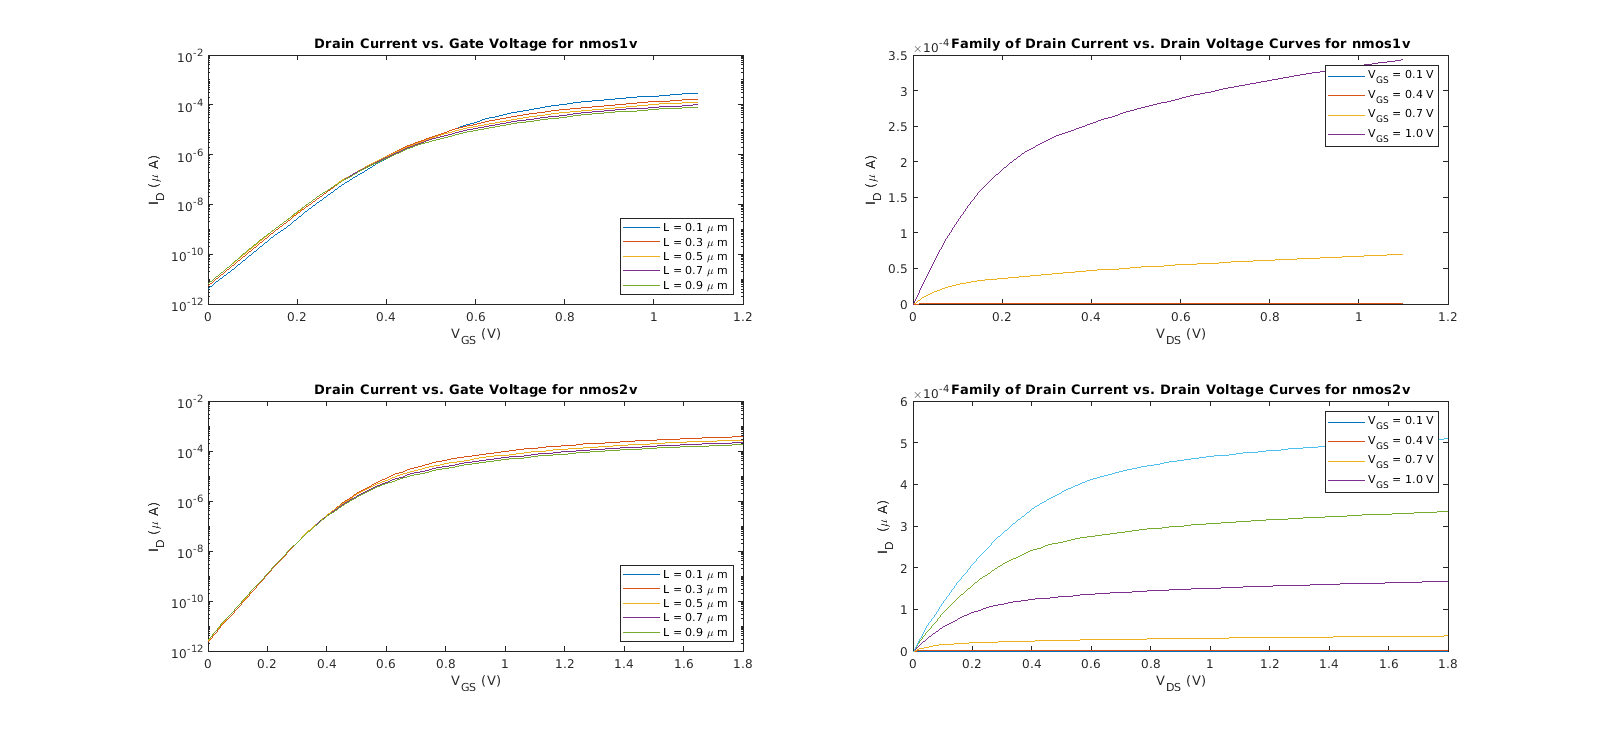
\includegraphics[scale=0.45, center]{plot1.PNG}\\
We can estimate the threshold voltage of each device by inspection.  The threshold voltage occurs when the $I_D - V_G$ curve stops being linear.
Below is the $V_{DS}$ for each device using the built-in functions in MATLAB, and the estimated threshold voltage.\\[0.25cm]
    \begin{table}[H]
    \centering
    \setlength{\tabcolsep}{20pt}
    \renewcommand{\arraystretch}{1.5}
        \begin{tabular}{|c|c|c|c|}
            \hline
            \textbf{Device} & $\text{Default}\;V_{DS}\,(V)$ & $\text{Maximum}\;V_{DS}\,(V)$ & $V_{Th}\,(V)$\\
            \hline
            \textit{nmos1v} & $0.55$ & $1.10$ & $0.375$\\
            \hline
            \textit{nmos2v} & $0.90$ & $1.80$ & $0.425$\\
            \hline
        \end{tabular}
    \end{table}
\newpage
%%%%%%%%%%%%%%%%%%%%%%%%%%%%%%%%%%%%%%%%%%%%%%%%%%%%%%
%                    QUESTION 2                      %
%%%%%%%%%%%%%%%%%%%%%%%%%%%%%%%%%%%%%%%%%%%%%%%%%%%%%%
\subsection{Question 2}
What is the length of the device in the $I_D - V_{DS}$ curves you just plotted?\\[0.5cm]
\underline{\textbf{\textit{Solution}}}\\[0.25cm]
Below is the $L$ for each device using the built-in functions in MATLAB.\\[0.25cm]
    \begin{table}[H]
    \centering
    \setlength{\tabcolsep}{20pt}
    \renewcommand{\arraystretch}{1.5}
        \begin{tabular}{|c|c|}
            \hline
            \textbf{Device} & $L\,(\mu m)$\\
            \hline
            \textit{nmos1v} & $0.05$\\
            \hline
            \textit{nmos2v} & $0.15$ \\
            \hline
        \end{tabular}
    \end{table}
%%%%%%%%%%%%%%%%%%%%%%%%%%%%%%%%%%%%%%%%%%%%%%%%%%%%%%
%                    QUESTION 3                      %
%%%%%%%%%%%%%%%%%%%%%%%%%%%%%%%%%%%%%%%%%%%%%%%%%%%%%%
\subsection{Question 3}
Draw the small signal model of an $NMOS$ and prove that:
\begin{equation}
    f_T \approx \frac{g_m}{2\pi c_{gg}}
\end{equation}
\begin{equation}
    c_{gg} = c_{gs} + c_{gd} + c_{bg}
\end{equation}
\underline{\textbf{\textit{Solution}}}\\[0.25cm]
On the following pages is the work of the small-signal model and proof.\\[0.25cm]
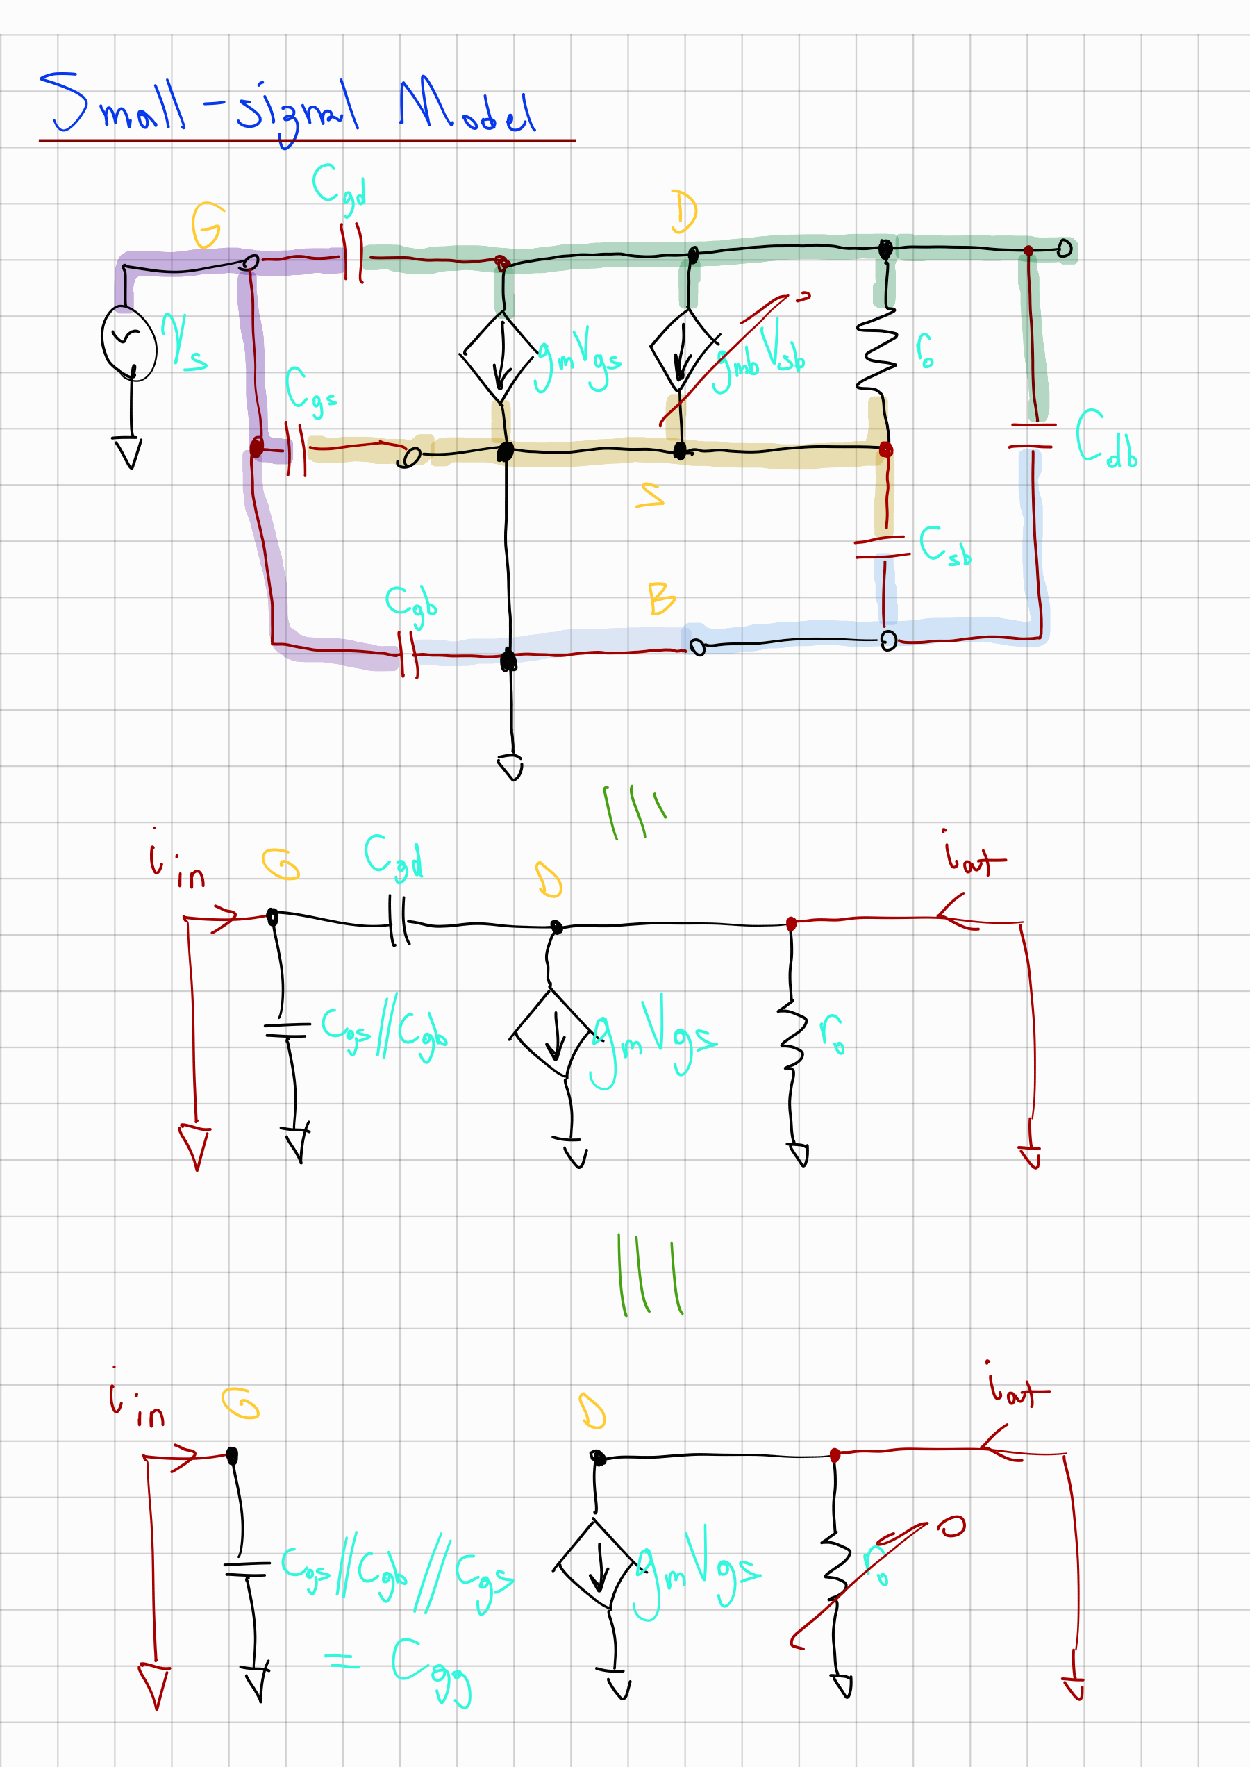
\includepdf[pages=1-2]{lab2_proof.PDF}
\newpage
%%%%%%%%%%%%%%%%%%%%%%%%%%%%%%%%%%%%%%%%%%%%%%%%%%%%%%
%                    QUESTION 4                      %
%%%%%%%%%%%%%%%%%%%%%%%%%%%%%%%%%%%%%%%%%%%%%%%%%%%%%%
\subsection{Question 4}
Plot $f_T$ and $A_v = g_m / g_{ds}$ of an intrinsic gain stage as a function of $g_m / I_D$.\\[0.5cm]
\underline{\textbf{\textit{Solution}}}\\[0.25cm]
Below is the plot:\\[0.25cm]
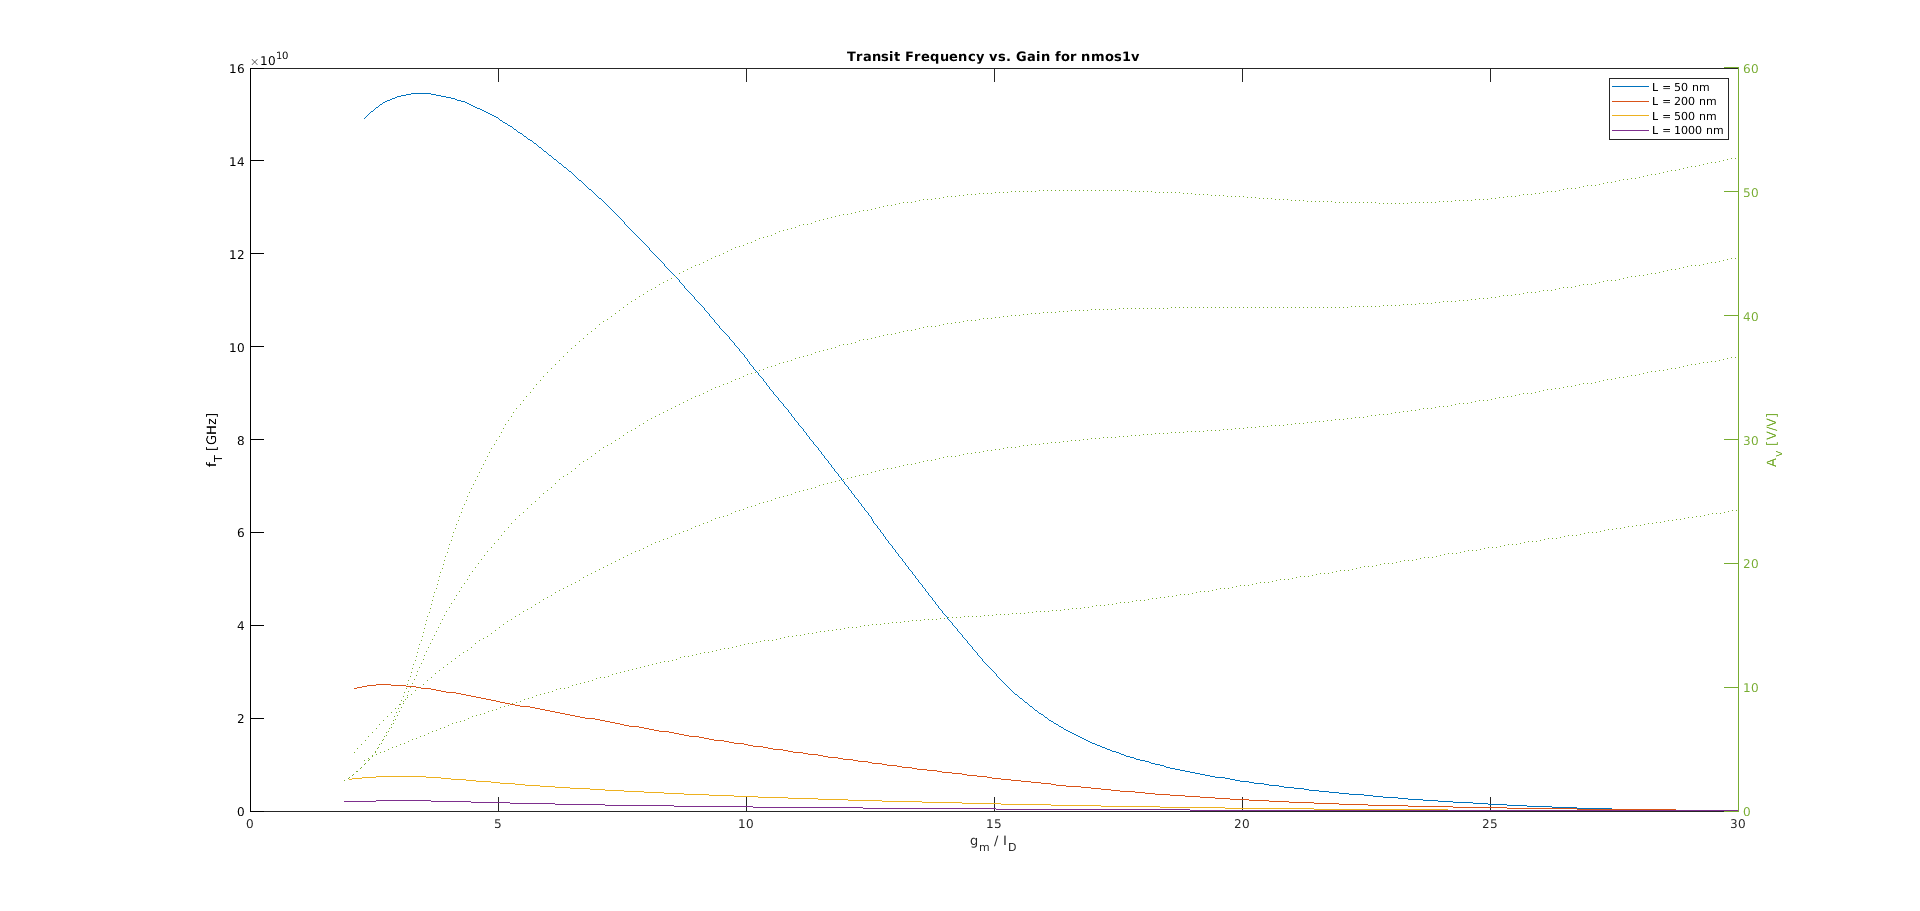
\includegraphics[scale=0.35, center]{plot2.PNG}\\
\newpage
%%%%%%%%%%%%%%%%%%%%%%%%%%%%%%%%%%%%%%%%%%%%%%%%%%%%%%%%%%%%%%%%%%%%%%%%%%%%%%%%%%%%%%%%%%%%%%%%%%%%%%%%%%%
%                                           LAB EXERCISES                                                 %
%%%%%%%%%%%%%%%%%%%%%%%%%%%%%%%%%%%%%%%%%%%%%%%%%%%%%%%%%%%%%%%%%%%%%%%%%%%%%%%%%%%%%%%%%%%%%%%%%%%%%%%%%%%
\newpage
\section{Lab Exercises}
In each exercise, a list of specifications are provided along with a semi-complete Matlab script.

You need to complete the Matlab script and verify your design in \textit{Cadence Virtuoso}. For each exercise, provide a table of comparison, comparing your simulated results with the specifications listed for that exercise.\\[0.5cm]
\newpage
%%%%%%%%%%%%%%%%%%%%%%%%%%%%%%%%%%%%%%%%%%%%%%%%%%%%%%
%                    EXERCISE 1                      %
%%%%%%%%%%%%%%%%%%%%%%%%%%%%%%%%%%%%%%%%%%%%%%%%%%%%%%
\subsection{Exercise 1: IGS with known $g_m / I_D$ and $L$}
\underline{\textbf{\textit{Solution}}}\\[0.25cm]
Below is a screenshot of the completed script in MATLAB, and the results of all parameters:\\[0.25cm]
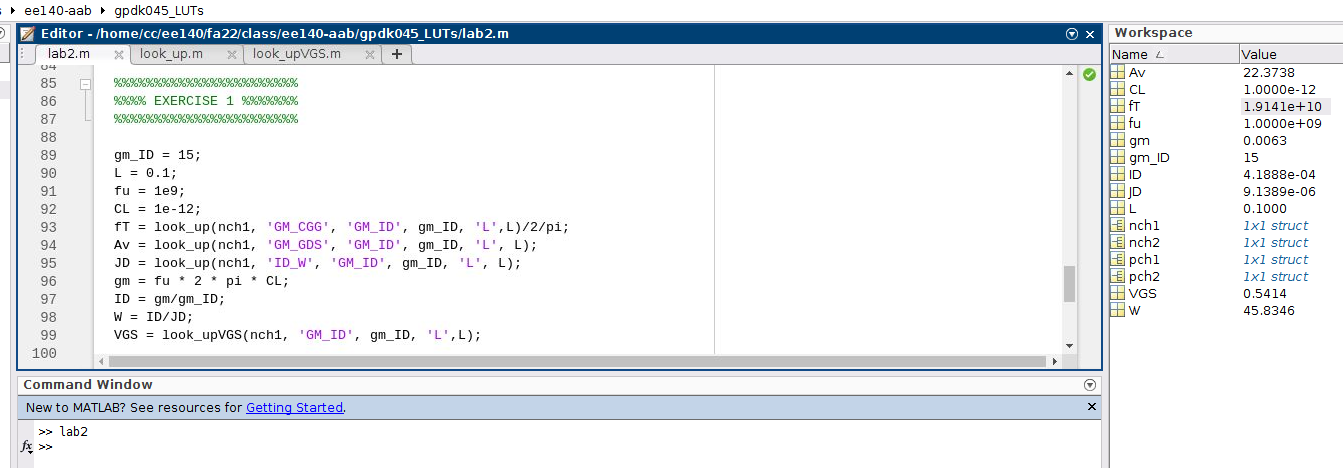
\includegraphics[scale=0.375, center]{mat_res1.PNG}\\[0.25cm]
Below is a schematic of the simulation in Cadence, with the DC node voltages shown.\\[0.25cm]
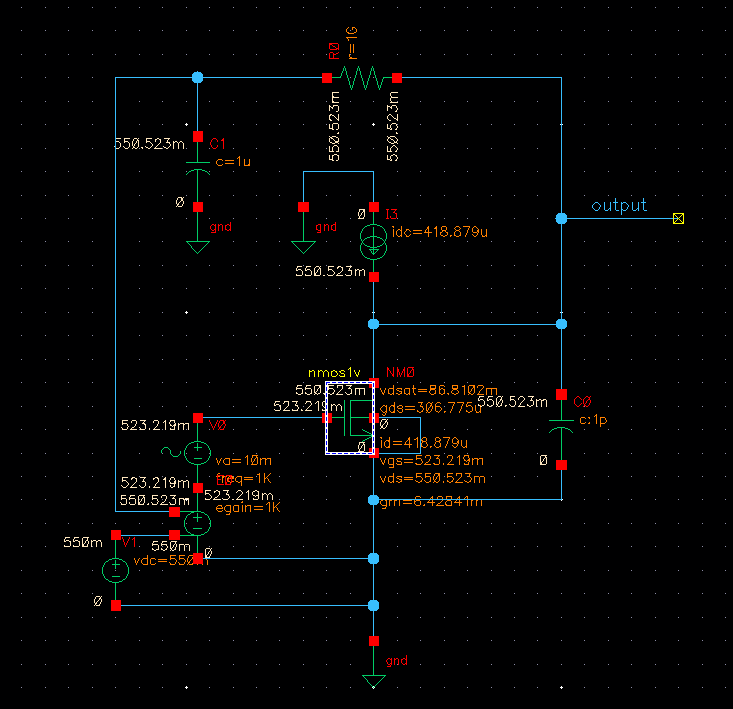
\includegraphics[scale=0.475, center]{schem1.PNG}\\[0.25cm]
\newpage
Below are the simulation results, and the Bode plot showing the unity gain frequency.\\[0.25cm]
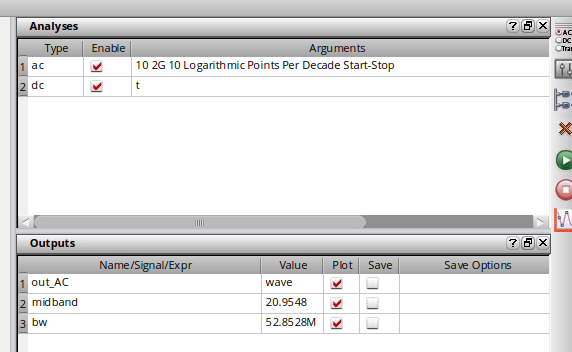
\includegraphics[scale=0.5, center]{sim_res1.PNG}\\[0.25cm]
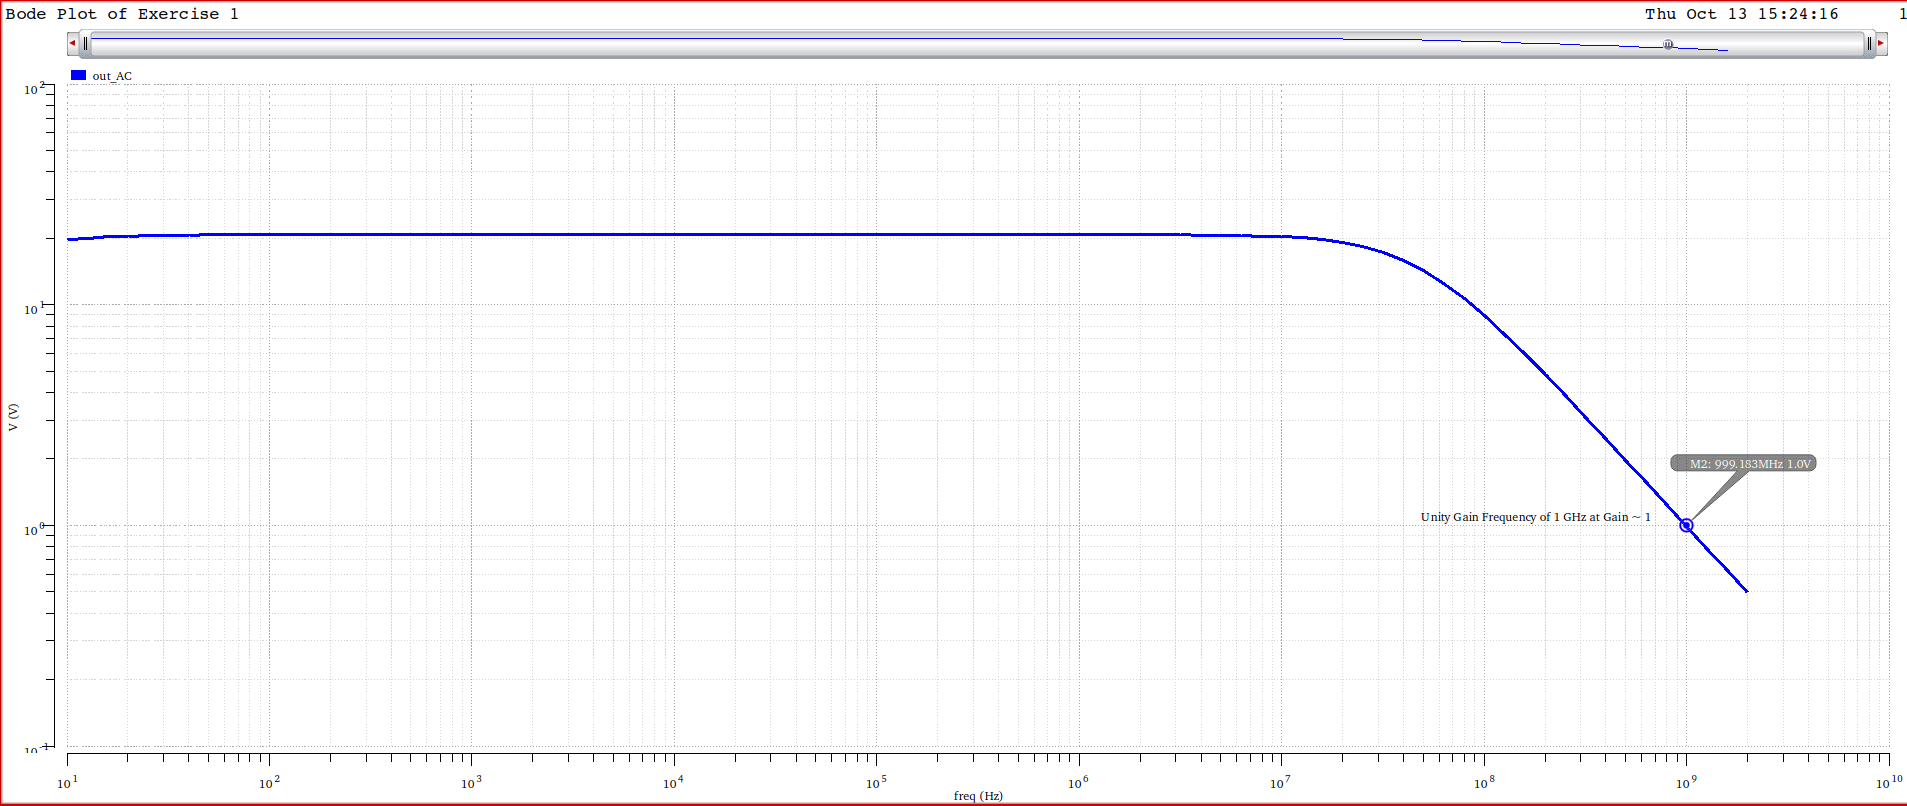
\includegraphics[scale=0.25, center]{bode1.PNG}\\[0.25cm]
Below is the table of results.  The simulated transconductance ratio was found using the DC operating point parameters table in Cadence.\\[0.25cm]
    \begin{table}[H]
    \centering
    \setlength{\tabcolsep}{20pt}
    \renewcommand{\arraystretch}{1.5}
        \begin{tabular}{|c|c|c|}
            \hline
            \textbf{Parameter} & \textit{Design} & \textit{Simulation}\\
            \hline
            Gain, $A_v\;(V/V)$ & $22.3738$ & $20.9548$\\
            \hline
            Unity Gain Bandwidth, $f_u\;(GHz)$ & $1.0$ & $0.999183$\\
            \hline
            Transconductance Ratio, $g_m / I_D\;({A\Omega}^{-1})$ & $15$ & $15.3467$\\
            \hline
            Gate Voltage, $V_{GS}\;(V)$ & $0.5414$ & $0.52321$\\
            \hline
        \end{tabular}
    \end{table}
\newpage
%%%%%%%%%%%%%%%%%%%%%%%%%%%%%%%%%%%%%%%%%%%%%%%%%%%%%%
%                    EXERCISE 2                      %
%%%%%%%%%%%%%%%%%%%%%%%%%%%%%%%%%%%%%%%%%%%%%%%%%%%%%%
\subsection{Exercise 2: IGS with known $g_m / I_D$, Variable $L$}
\underline{\textbf{\textit{Solution}}}\\[0.25cm]
Below is a screenshot of the completed script in MATLAB, and the results of all parameters.  The parameters were pasted into one spreadsheet for ease of matching the indices.  The row corresponding to the minimum transition frequency is highlighted.\\[0.25cm]
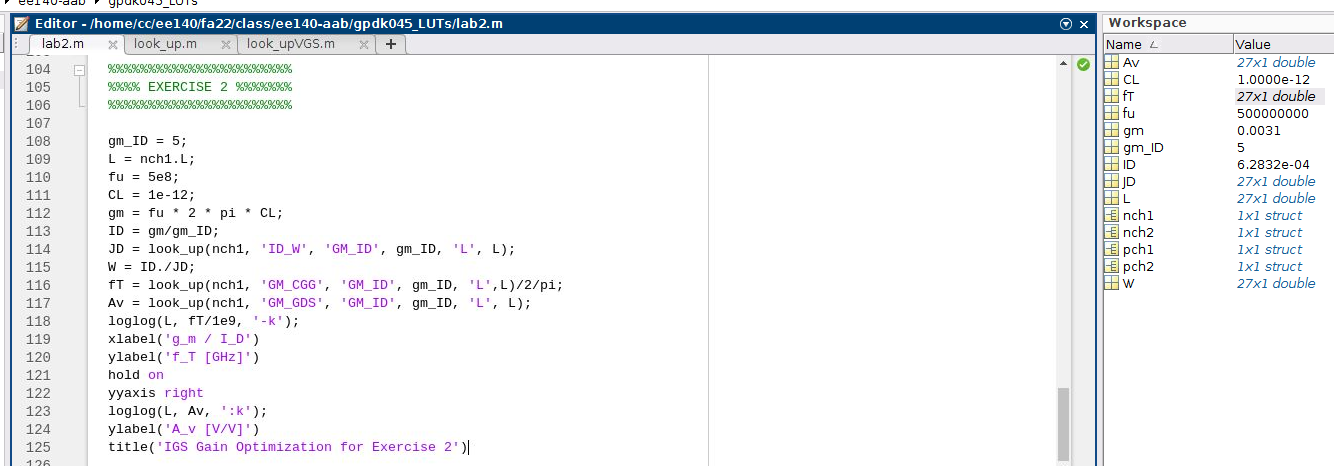
\includegraphics[scale=0.375, center]{mat_res2.PNG}\\[0.25cm]
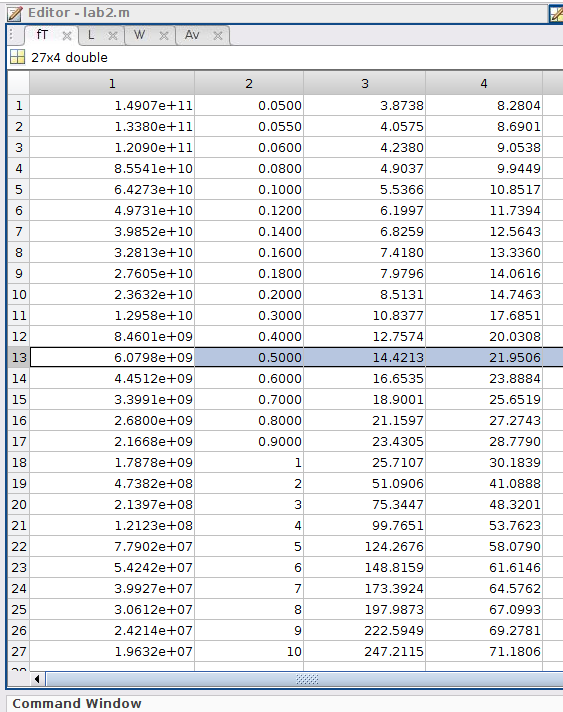
\includegraphics[scale=0.475, center]{mat_res3.PNG}\\[0.25cm]
\newpage
\noindent
Below is a plot of the IGS gain optimization curve.\\[0.25cm]
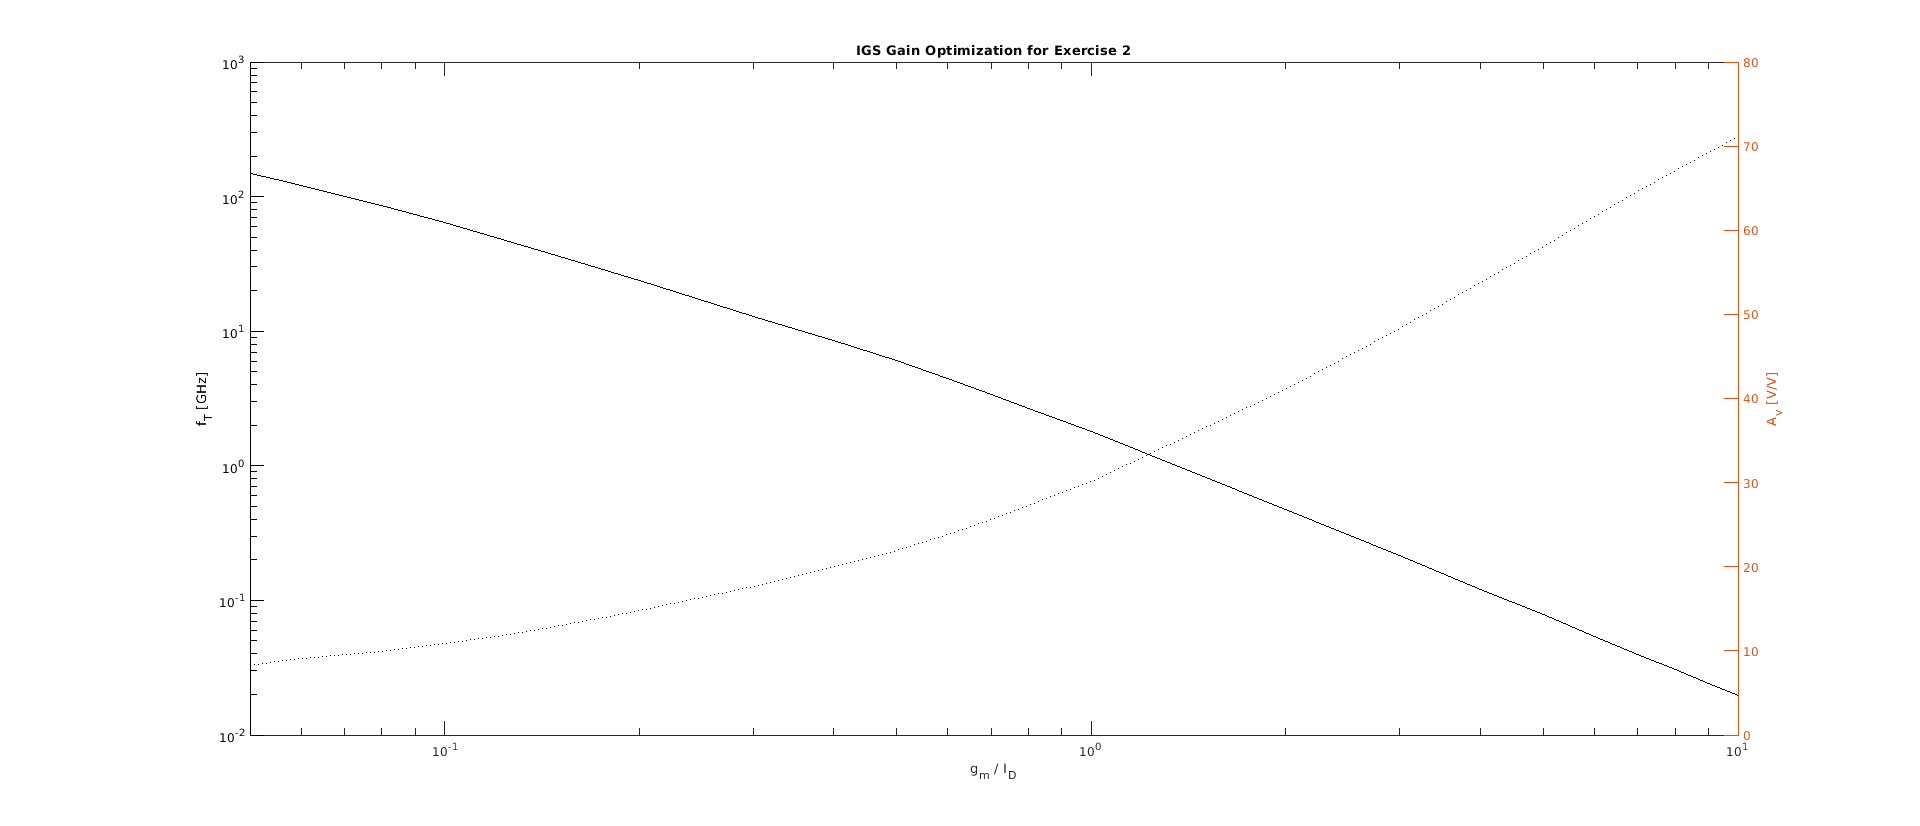
\includegraphics[scale=0.375, center]{plot3.PNG}\\[0.25cm]
Since we have the constraint that $f_u \leq f_T/10$, we must choose a transition frequency greater than $\approx 5\,GHz$ and the corresponding length and width for two solution sets.  We can also find that maximum length for $L$ based on its correspondance with the first valid transition frequency, as indicated on row 13 from the previous spreadsheet image:
\begin{equation}
    \boxed{L_{MAX} = 0.5 \mu m}
\end{equation}
Based on the results in MATLAB, we are using these two sets of solutions to use for the simulations in Cadence.
    \begin{table}[H]
    \centering
    \setlength{\tabcolsep}{20pt}
    \renewcommand{\arraystretch}{1.5}
        \begin{tabular}{|c|c|c|}
            \hline
            \textbf{Parameter} & \textit{Solution Set 1} & \textit{Solution Set 2}\\
            \hline
            $f_T\;(GHz)$ & $1.4907$ & $1.2958$\\
            \hline
            $W\;(\mu m)$ & $3.8738$ & $10.8377$\\
            \hline
            $L\;(\mu m)$ & $0.05$ & $0.3$\\
            \hline
            $A_v\;(V/V)$ & $8.2804$ & $17.6851$\\
            \hline
        \end{tabular}
    \end{table}
\newpage
\noindent
Below is a schematic of the first simulation in Cadence, with the DC node voltages shown.\\[0.25cm]
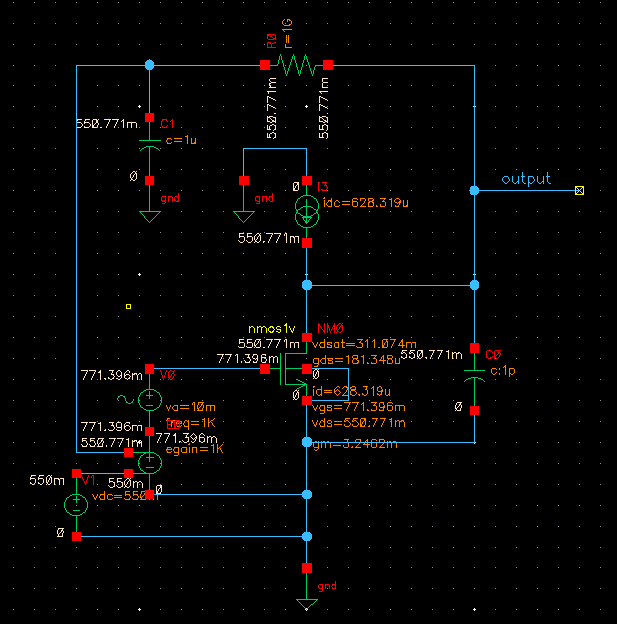
\includegraphics[scale=0.5, center]{schem2.PNG}\\[0.25cm]
Below are the results of the first simulation.\\[0.25cm]
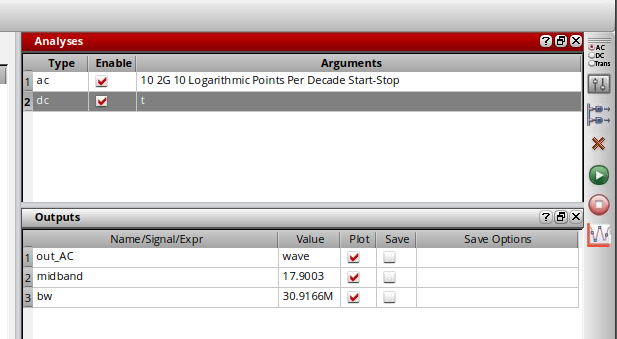
\includegraphics[scale=0.55, center]{sim_res2.PNG}\\[0.25cm]
\newpage
\noindent
Below is a schematic of the second simulation in Cadence, with the DC node voltages shown.\\[0.25cm]
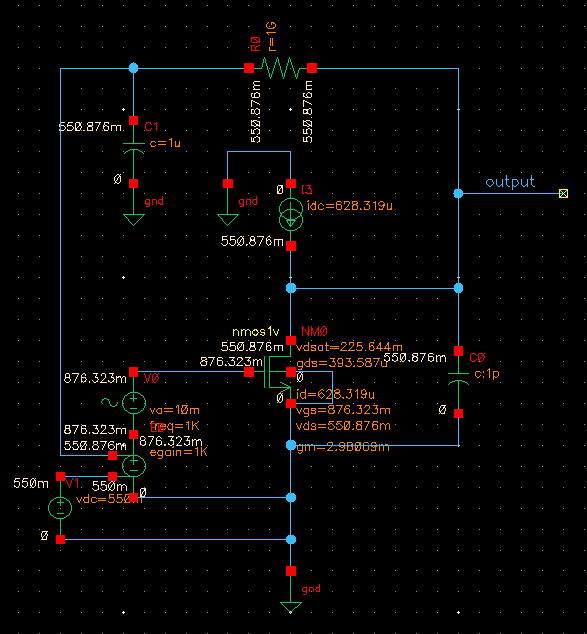
\includegraphics[scale=0.5, center]{schem3.PNG}\\[0.25cm]
Below are the results of the second simulation.\\[0.25cm]
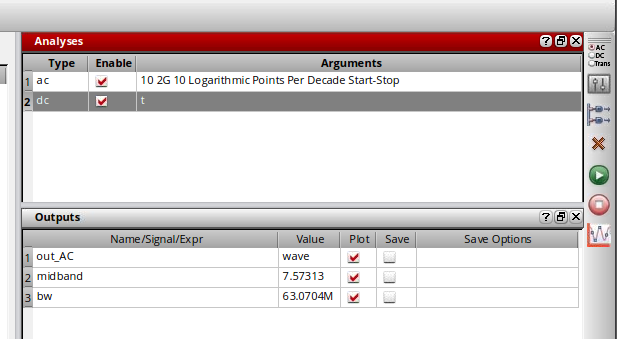
\includegraphics[scale=0.55, center]{sim_res3.PNG}\\[0.25cm]
\newpage\noindent
Below is the Bode plot with the unity gain frequency marked for the parameters using the first solution.\\[0.25cm]
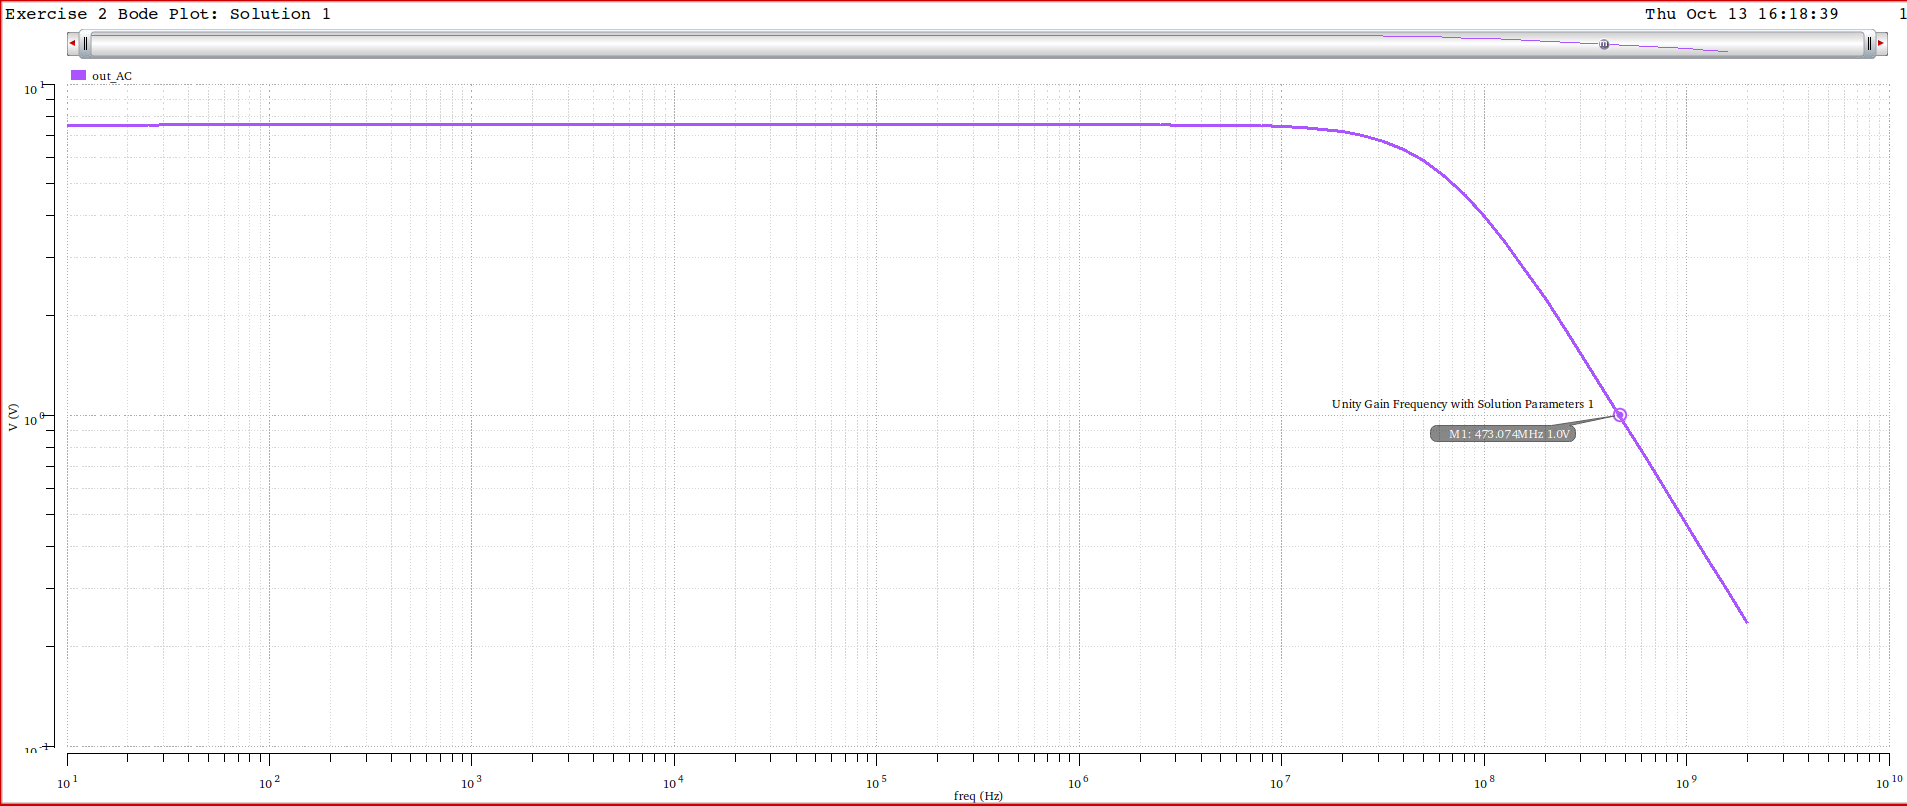
\includegraphics[scale=0.25, center]{bode2.PNG}\\[0.25cm]
Below is the Bode plot with the unity gain frequency marked for the parameters using the second solution.\\[0.25cm]
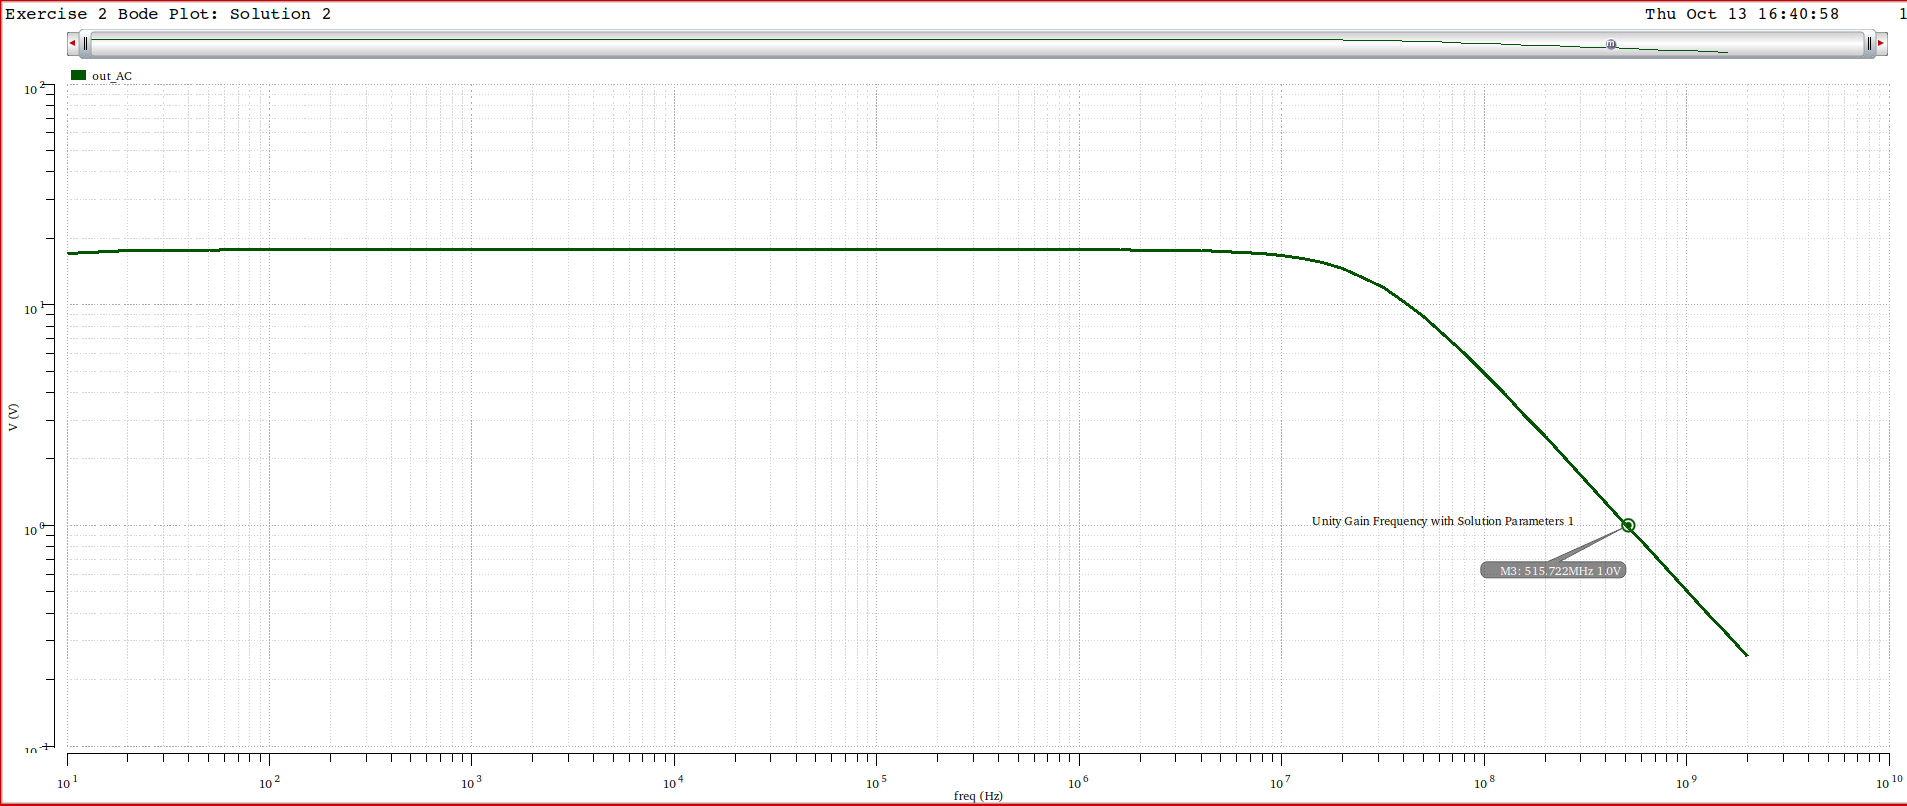
\includegraphics[scale=0.25, center]{bode3.PNG}\\[0.25cm]
Both solutions are close to $500\,MHz$ and confirm that they both obtain $f_U$.\\[0.25cm]
\newpage\noindent
Below is a table comparing the performance results.
    \begin{table}[H]
    \centering
    \setlength{\tabcolsep}{20pt}
    \renewcommand{\arraystretch}{1.5}
        \begin{tabular}{|c|c|c|}
            \hline
            \textbf{Parameter} & \textit{Solution Set 1} & \textit{Solution Set 2}\\
            \hline
            Gain, $A_v\;(V/V)$ & $7.57313$ & $17.9003$\\
            \hline
            Bandwidth, $BW\;(MHz)$ & $63.0704$ & $30.916$\\
            \hline
            Unity Gain Bandwidth $f_u\;(MHz)$ & $473.074$ & $515.722$\\
            \hline
            Transconductance Ratio, $g_m / I_D\;({A\Omega}^{-1})$ & $4.74319$ & $5.16649$\\
            \hline
            Gate Voltage, $V_{GS}\;(V)$ & $0.876$ & $0.771$\\
            \hline
        \end{tabular}
    \end{table}
\newpage
%%%%%%%%%%%%%%%%%%%%%%%%%%%%%%%%%%%%%%%%%%%%%%%%%%%%%%
%                    EXERCISE 3                      %
%%%%%%%%%%%%%%%%%%%%%%%%%%%%%%%%%%%%%%%%%%%%%%%%%%%%%%
\subsection{Exercise 3: IGS with Variable $g_m / I_D$ and $L$, Max $A_v$ Optimization}
Below is the MATLAB code:\\[0.25cm]
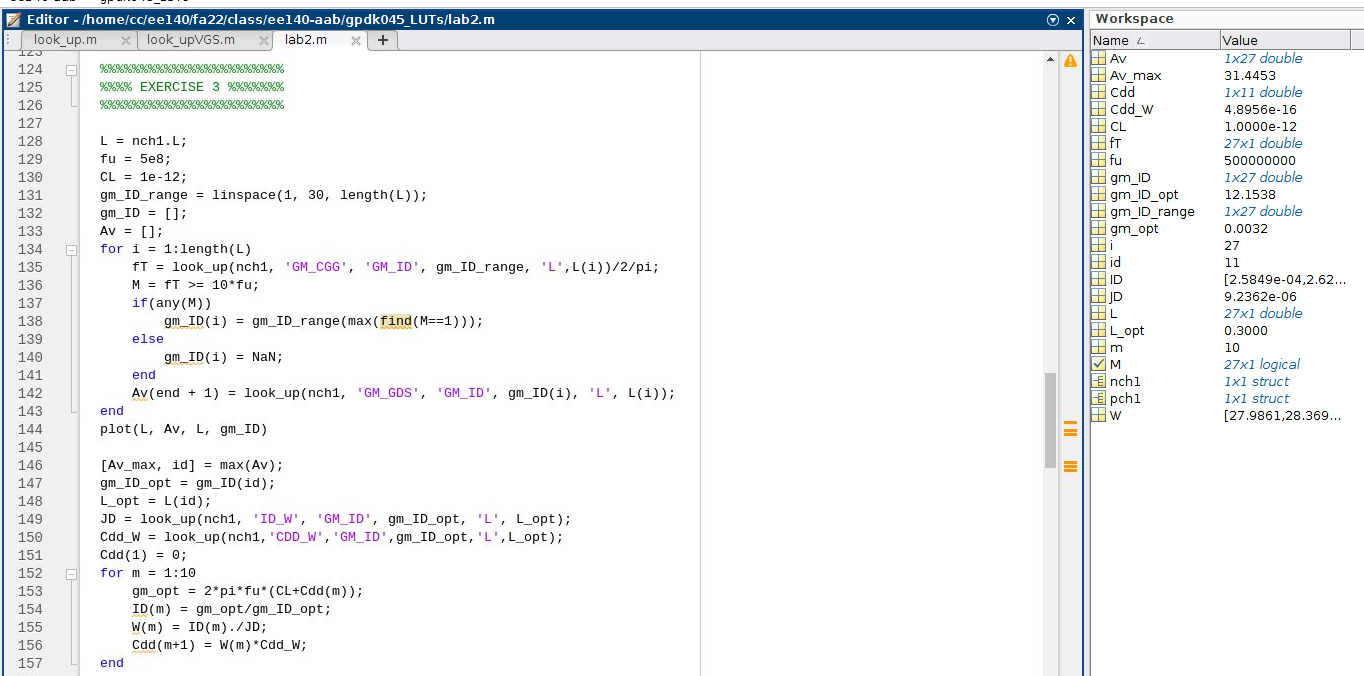
\includegraphics[scale=0.375, center]{mat_res4.PNG}\\[0.25cm]
Below is the accompanying plot:\\[0.25cm]
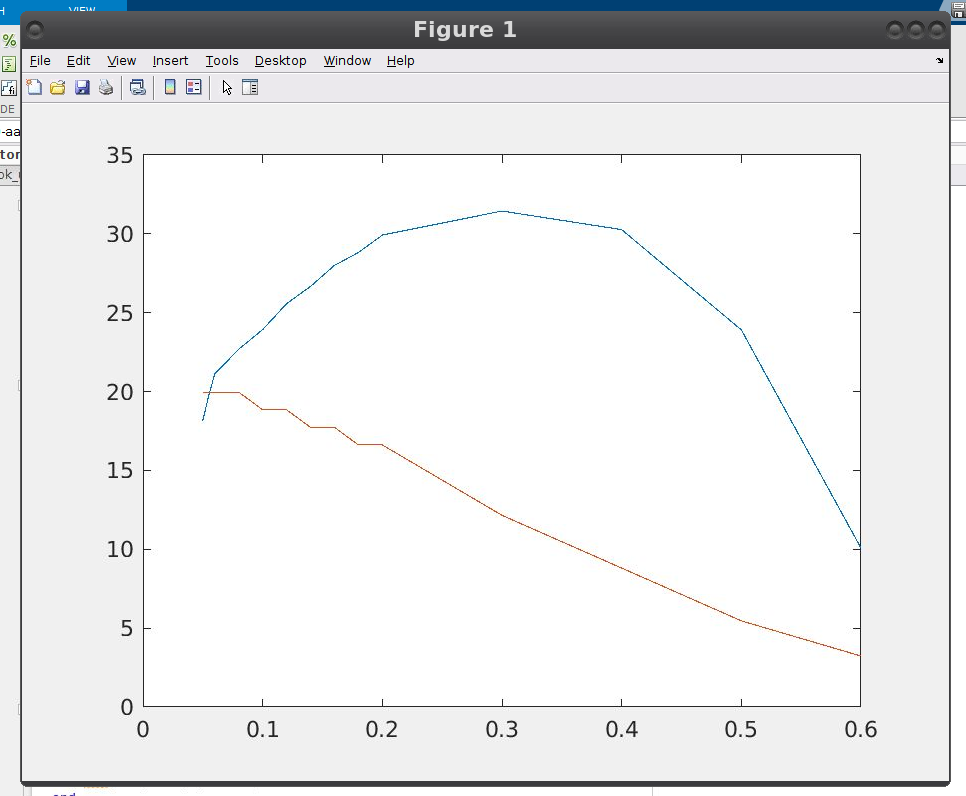
\includegraphics[scale=0.375, center]{mat_res5.PNG}\\[0.25cm]
The schematic remains unchanged.  Below is the results of the simulation using the results from MATLAB:\\[0.25cm]
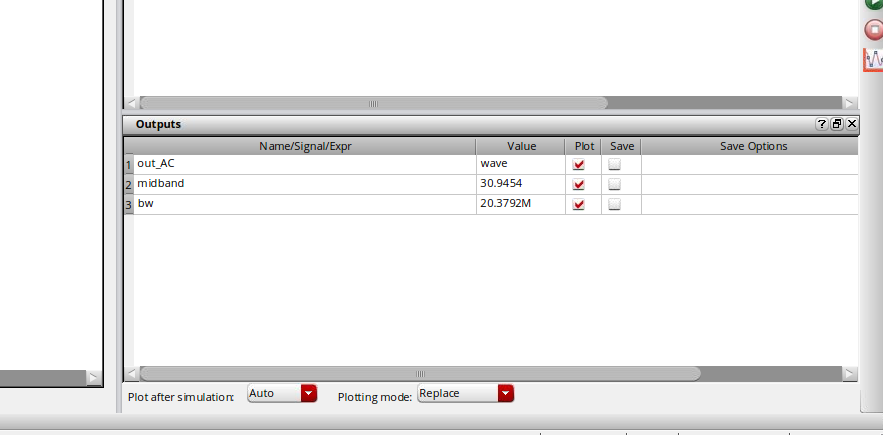
\includegraphics[scale=0.375, center]{sim_res4.PNG}\\[0.25cm]
Below is the Bode plot:\\[0.25cm]
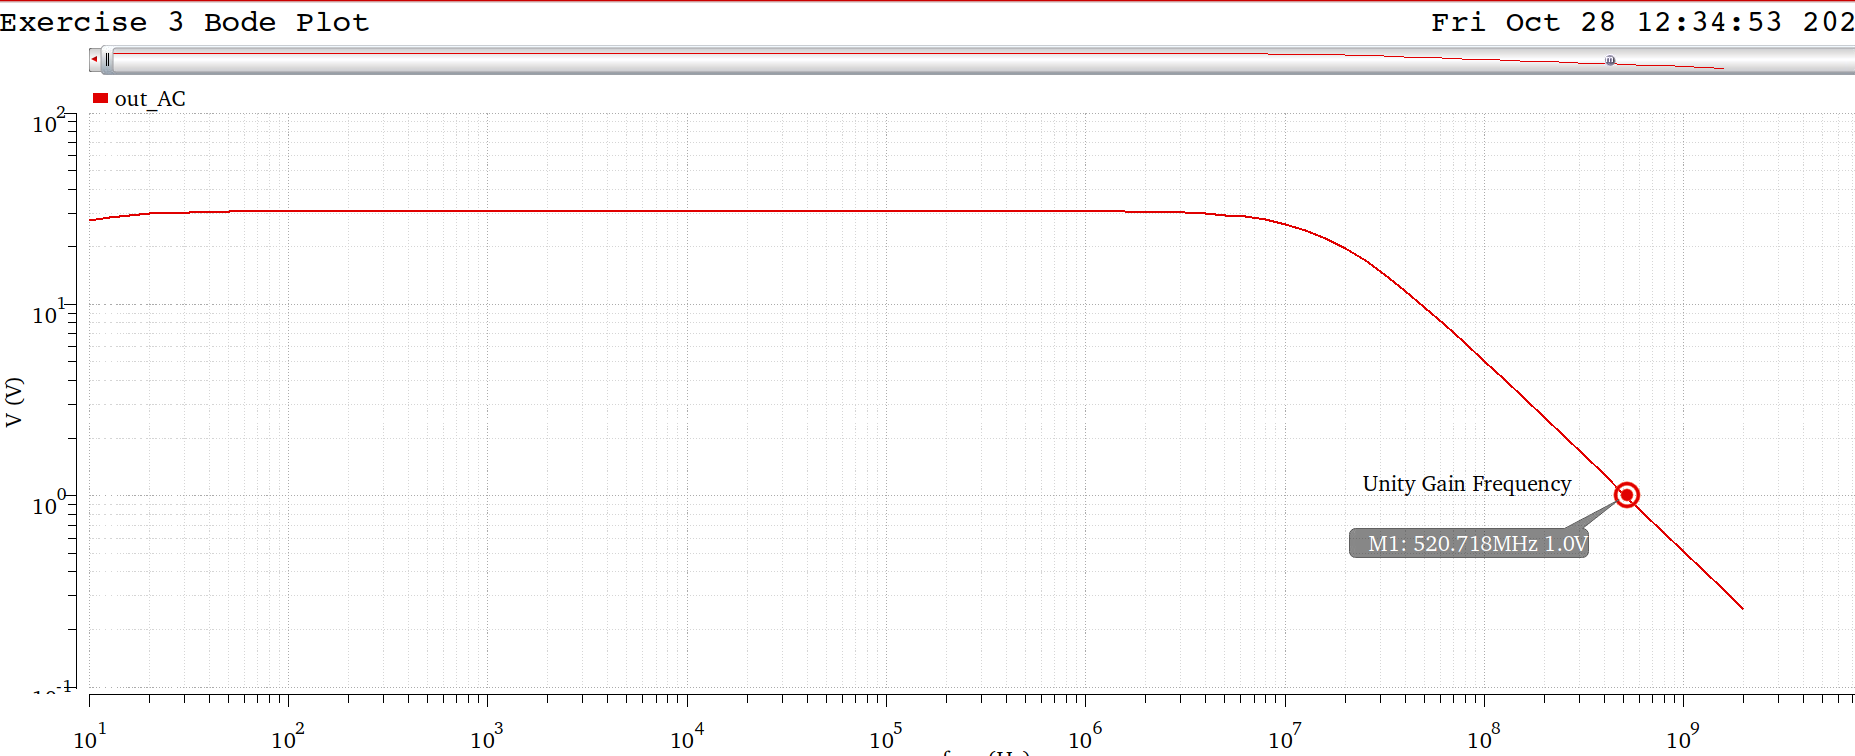
\includegraphics[scale=0.275, center]{bode4.PNG}\\[0.25cm]
Below is a table of the performance results in this experiment compared to the results of \textit{Ex.(2)}.
    \begin{table}[H]
    \centering
    \setlength{\tabcolsep}{12pt}
    \renewcommand{\arraystretch}{1.25}
        \begin{tabular}{|c|c|c|c|}
            \hline
            \textbf{Parameter} & \textit{Ex.(3) Simulation} & \textit{Ex.(2) Solution Set 1} & \textit{Ex.(2) Solution Set 2}\\
            \hline
            $A_v\;(V/V)$ & $30.9454$ & $7.57313$ & $17.9003$\\
            \hline
            $BW\;(MHz)$ & $20.3792$ & $63.0704$ & $30.916$\\
            \hline
            $f_u\;(MHz)$ & $520.718$ & $473.074$ & $515.722$\\
            \hline
            $g_m / I_D\;({A\Omega}^{-1})$ & $12.5651$ & $4.74319$ & $5.16649$\\
            \hline
            $V_{GS}\;(V)$ & $0.539$ & $0.876$ & $0.771$\\
            \hline
        \end{tabular}
    \end{table}
\newpage
%%%%%%%%%%%%%%%%%%%%%%%%%%%%%%%%%%%%%%%%%%%%%%%%%%%%%%
%                    EXERCISE 4                      %
%%%%%%%%%%%%%%%%%%%%%%%%%%%%%%%%%%%%%%%%%%%%%%%%%%%%%%
\subsection{Exercise 4: Common-source with active $PMOS$ load / classic differentia design}
Below is the MATLAB code:\\[0.25cm]
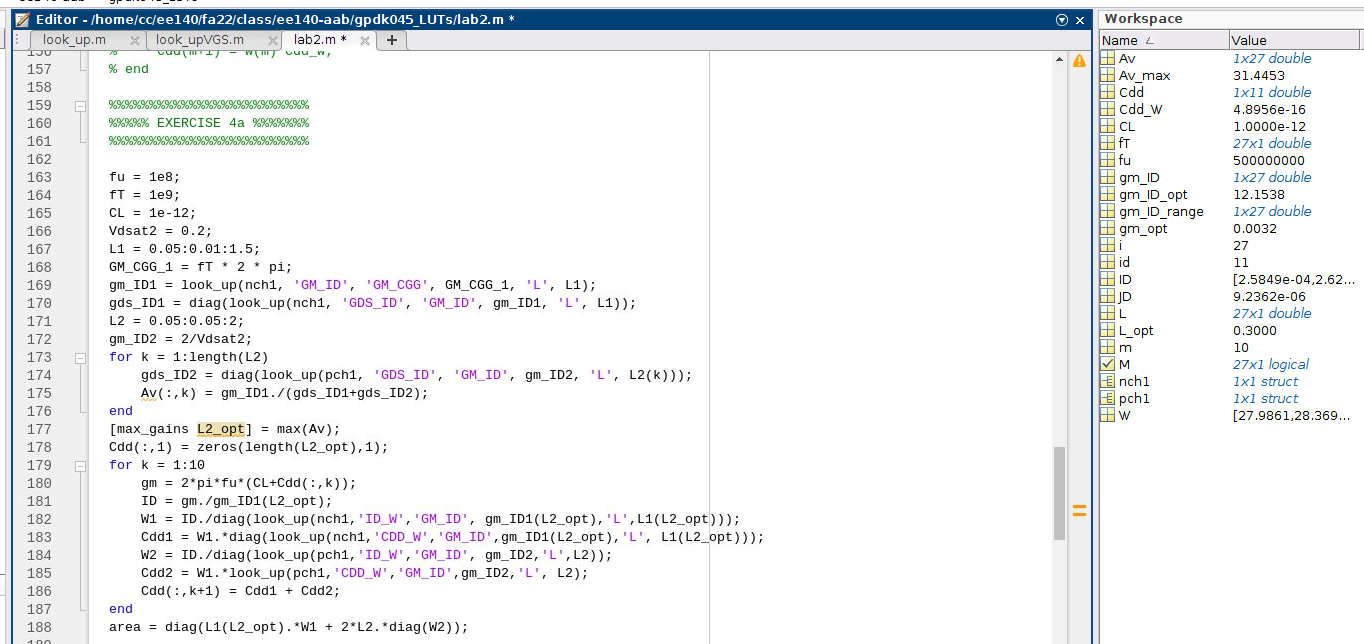
\includegraphics[scale=0.35, center]{mat_res6.PNG}\\[0.25cm]
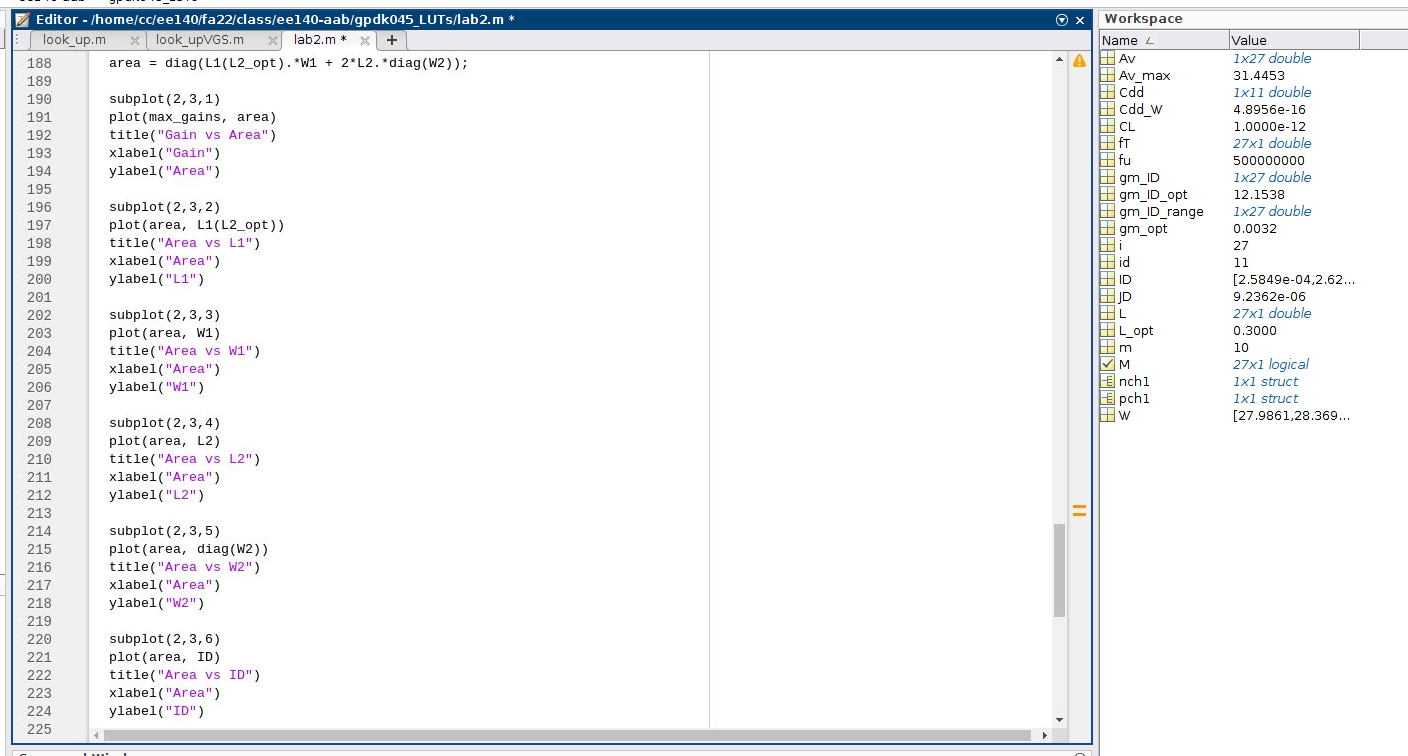
\includegraphics[scale=0.35, center]{mat_res7.PNG}\\[0.25cm]
\newpage
Below are the plots used to find the optimal parameters for simulation.  The gain is 25.0615, and the area is 14.7507.:\\[0.25cm]
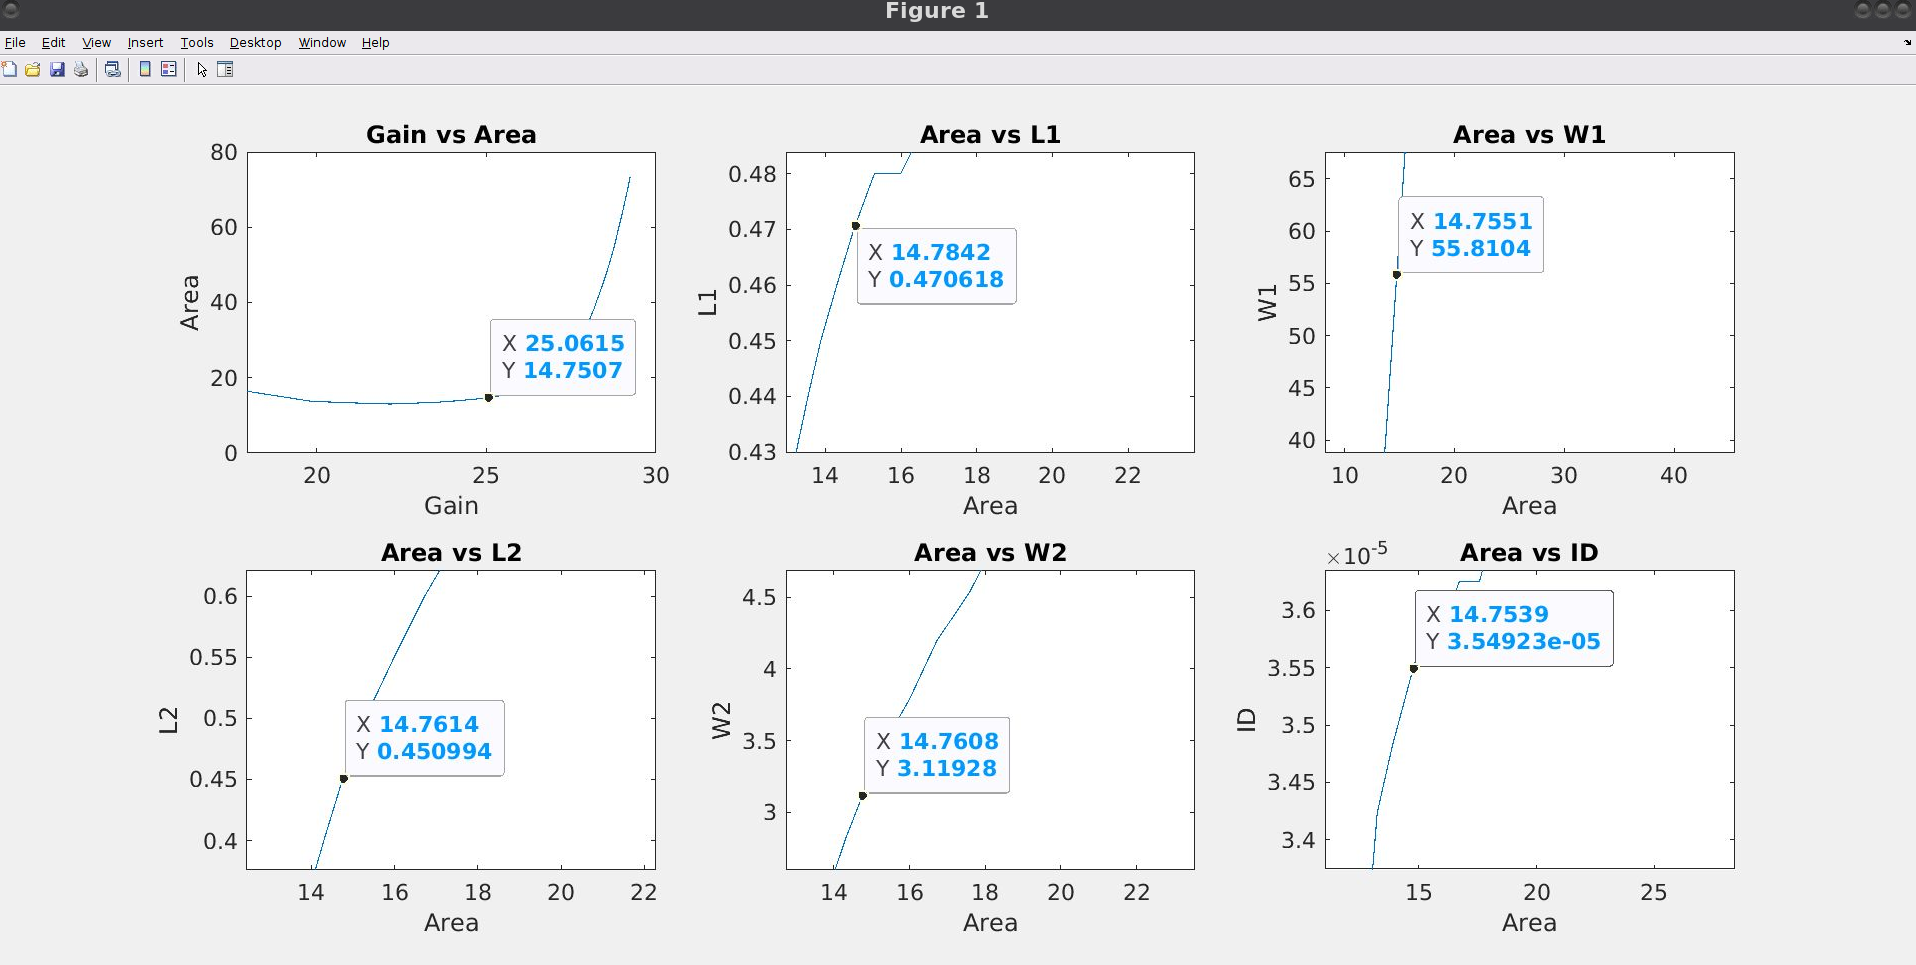
\includegraphics[scale=0.275, center]{mat_res8.PNG}\\[0.25cm]
Below is the schematic in Cadence:\\[0.25cm]
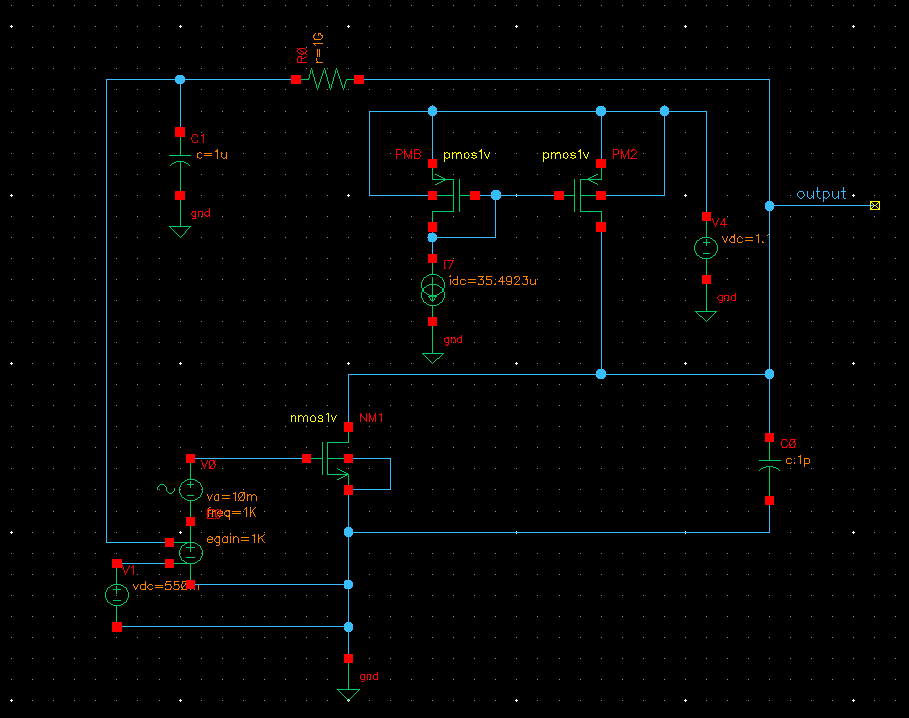
\includegraphics[scale=0.325, center]{schem4.PNG}\\[0.25cm]
\newpage
Below is the results of the simulation using the results from MATLAB:\\[0.25cm]
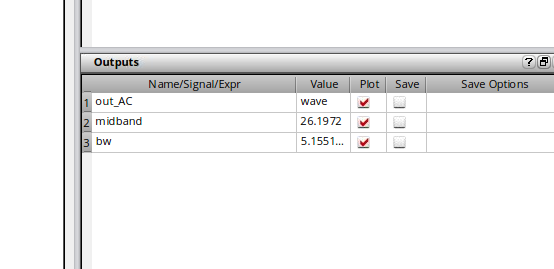
\includegraphics[scale=0.475, center]{sim_res5.PNG}\\[0.25cm]
Below is the Bode plot:\\[0.25cm]
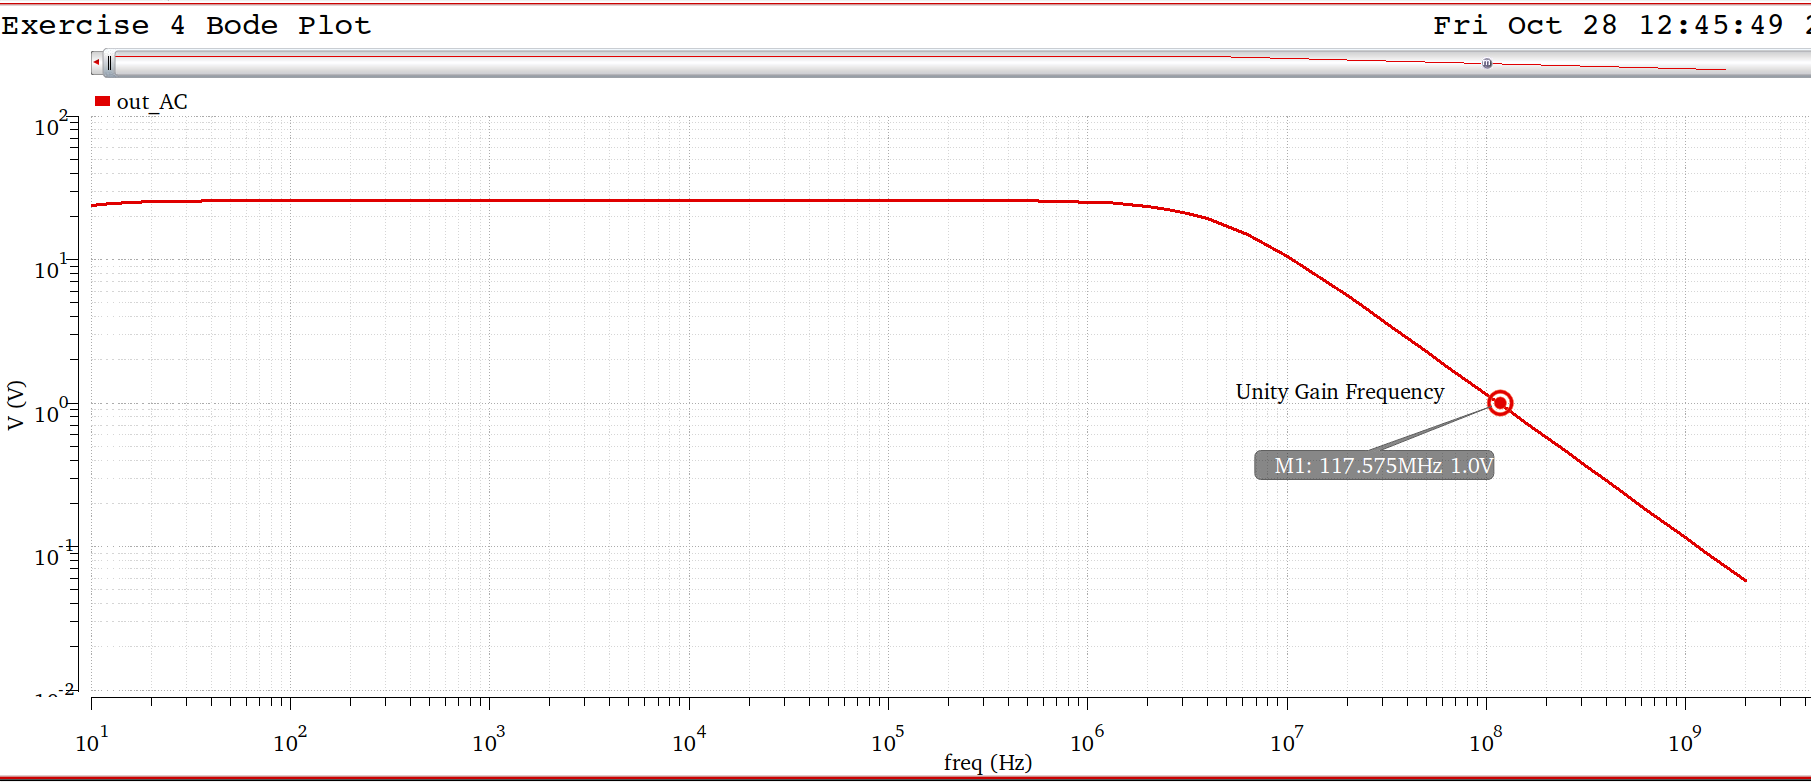
\includegraphics[scale=0.275, center]{bode5.PNG}\\[0.25cm]
Below is a table comparing the calculations in MATLAB to the simulation in Cadence:\\[0.25cm]
    \begin{table}[H]
    \centering
    \setlength{\tabcolsep}{4pt}
    \renewcommand{\arraystretch}{1.5}
        \begin{tabular}{|c|c|c|}
            \hline
            \textbf{Parameter} & \textit{Calculations} & \textit{Simulation}\\
            \hline
            $A_v\;(V/V)$ & $25.0615$ & $26.1972$\\
            \hline
            $g_m / I_D\;({A\Omega}^{-1})$ & $22.8809$ & $21.1049$\\
            \hline
            $f_u\;(MHz)$ & $100$ & $117.575$\\
            \hline
        \end{tabular}
    \end{table}
\newpage
Below is a screenshot of the schematic in Cadence converted to a differential circuit.  The node voltages are included, and the DC values were swept in order to find the proper biasing points for the current and voltage sources:\\[0.25cm]
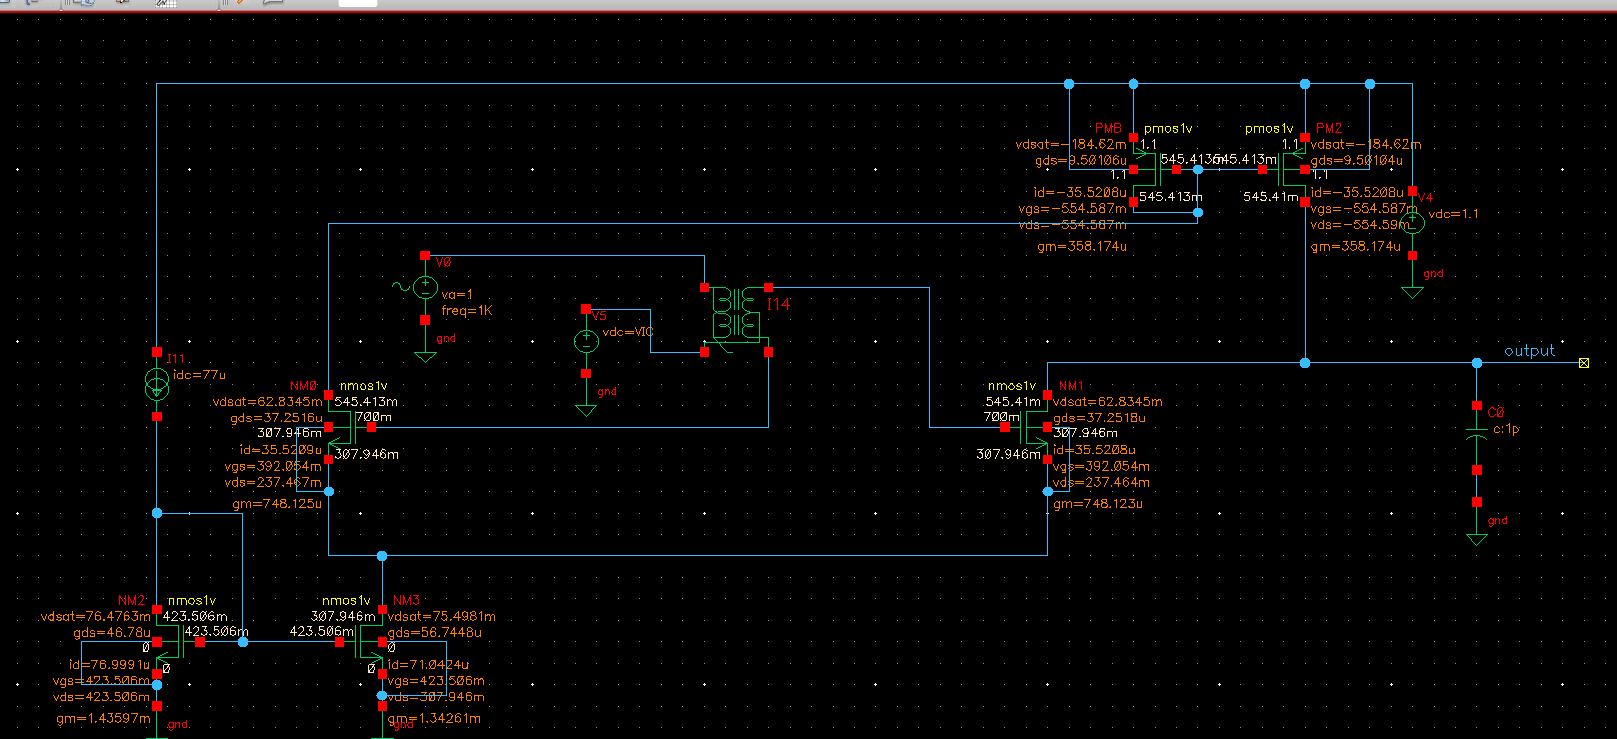
\includegraphics[scale=0.35, center]{schem5.PNG}\\[0.25cm]
Below is the new results of the simulation using the results from MATLAB:\\[0.25cm]
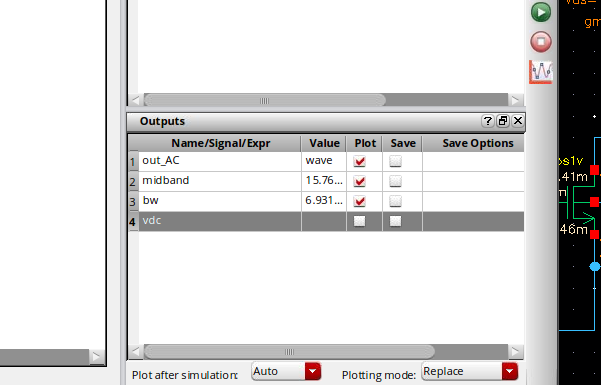
\includegraphics[scale=0.475, center]{sim_res6.PNG}\\[0.25cm]
\newpage
Below is the new Bode plot:\\[0.25cm]
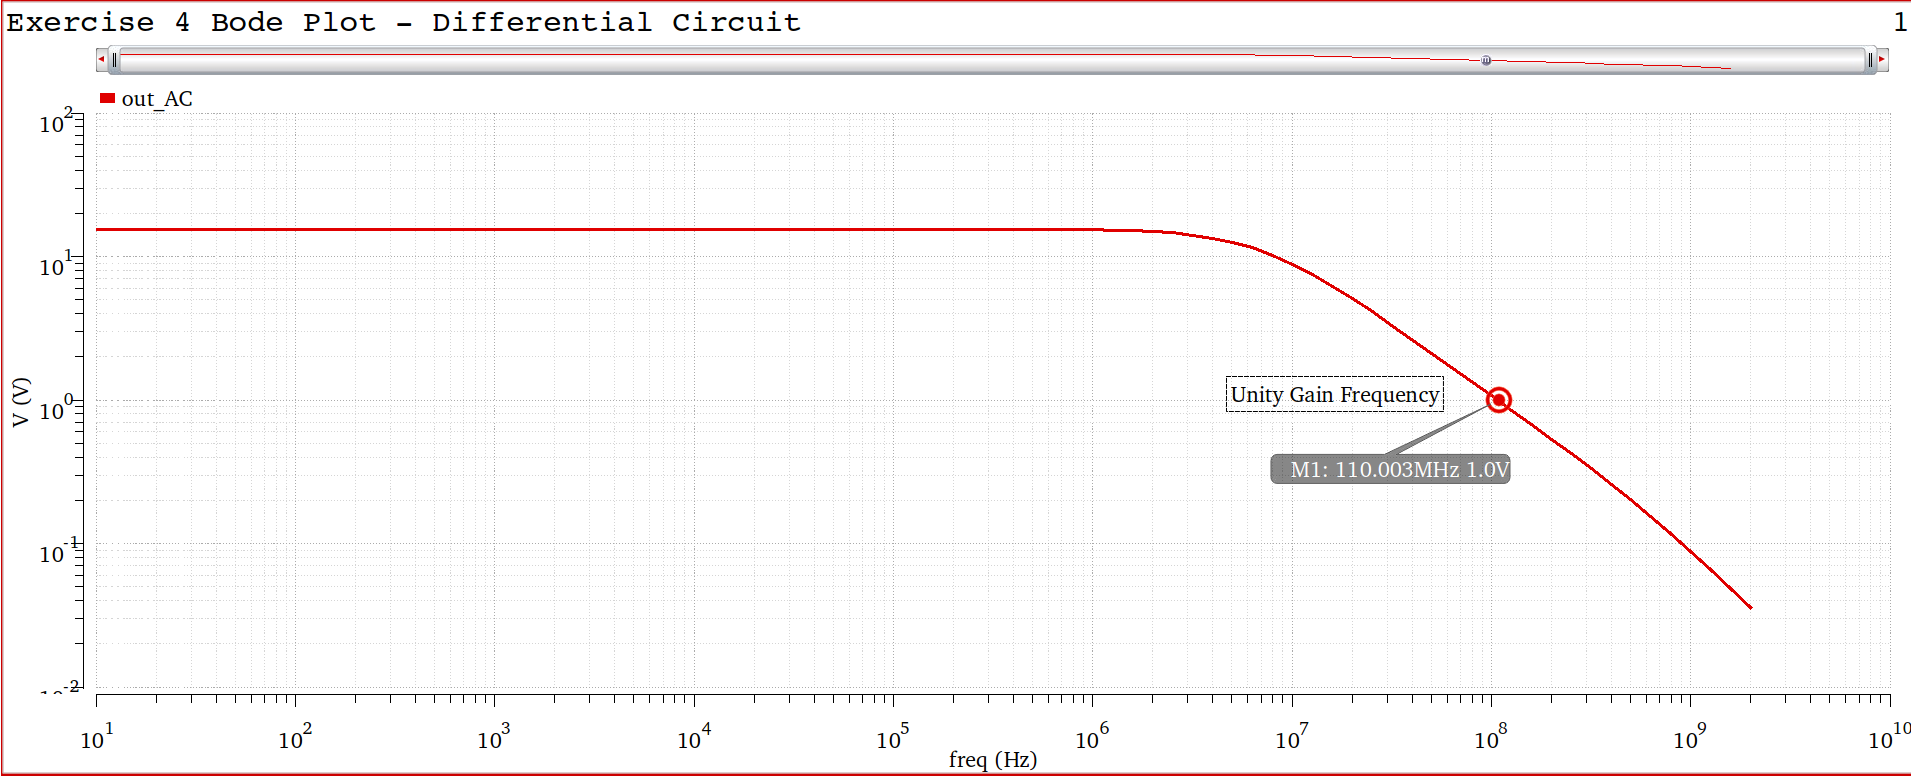
\includegraphics[scale=0.275, center]{bode6.PNG}\\[0.25cm]
Below is a table comparing the performance results of both designs:
    \begin{table}[H]
    \centering
    \setlength{\tabcolsep}{20pt}
    \renewcommand{\arraystretch}{1.5}
        \begin{tabular}{|c|c|c|}
            \hline
            \textbf{Parameter} & \textit{Ex. 4a} & \textit{Ex. 4b}\\
            \hline
            $A_v\;(V/V)$ & $26.1972$ & $15.76$\\
            \hline
            $BW\;(MHz)$ & $5.155$ & $6.931$\\
            \hline
            $f_u\;(MHz)$ & $117.575$ & $110.003$\\
            \hline
            $g_m / I_D\;({A\Omega}^{-1})$ & $21.1049$ & $21.0615$\\
            \hline
        \end{tabular}
    \end{table}
\newpage
%%%%%%%%%%%%%%%%%%%%%%%%%%%%%%%%%%%%%%%%%%%%%%%%%%%%%%
%                    EXERCISE 5                      %
%%%%%%%%%%%%%%%%%%%%%%%%%%%%%%%%%%%%%%%%%%%%%%%%%%%%%%
\subsection{Exercise 5}
Below is the schematic in Cadence of the amplifier with the given specs:\\[0.25cm]
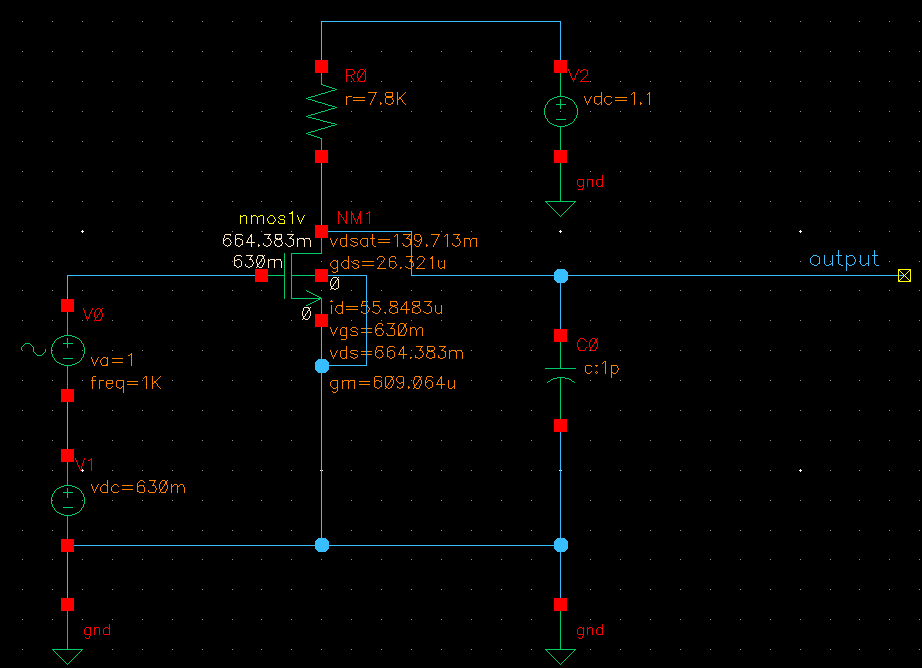
\includegraphics[scale=0.25, center]{schem6.PNG}\\[0.25cm]
Below is the results of the simulation using the results from MATLAB:\\[0.25cm]
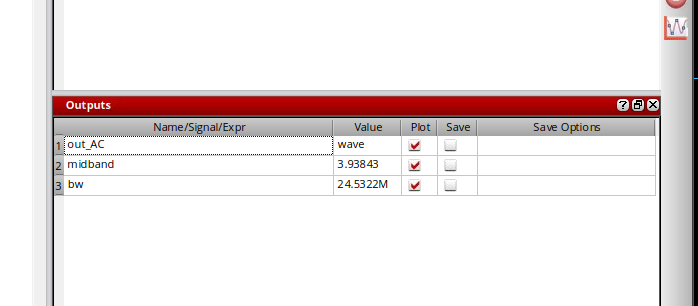
\includegraphics[scale=0.275, center]{sim_res7.PNG}\\[0.25cm]
Below is the Bode plot with the unity gain frequency marked:\\[0.25cm]
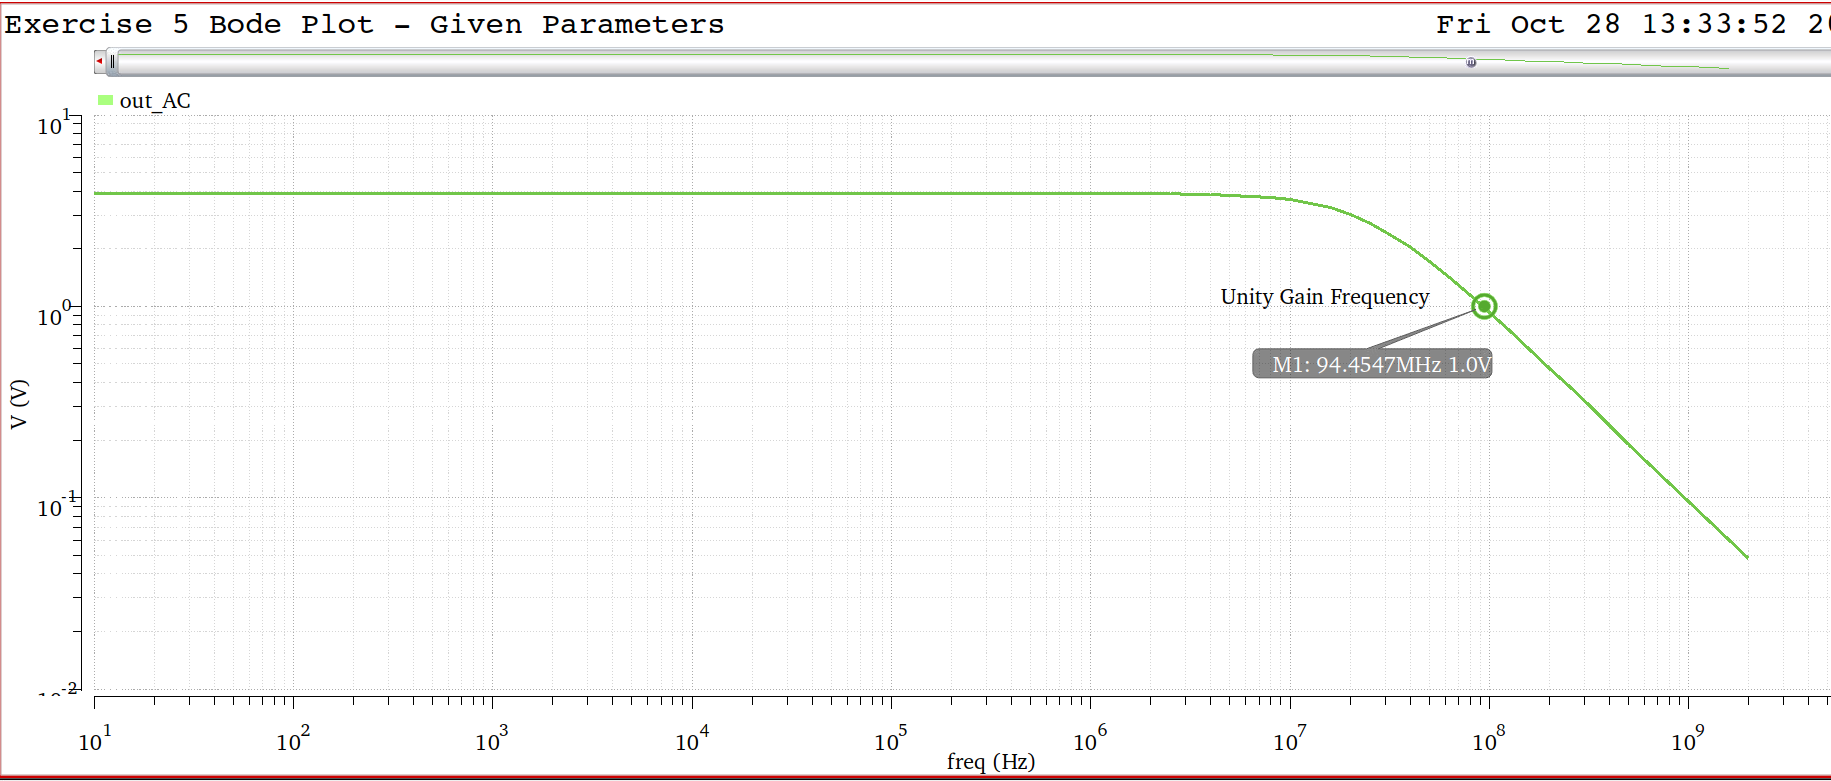
\includegraphics[scale=0.275, center]{bode7.PNG}\\[0.25cm]
\newpage
Below is the MATLAB code for the amplifier with $f_u = 1\;GHz$:\\[0.25cm]
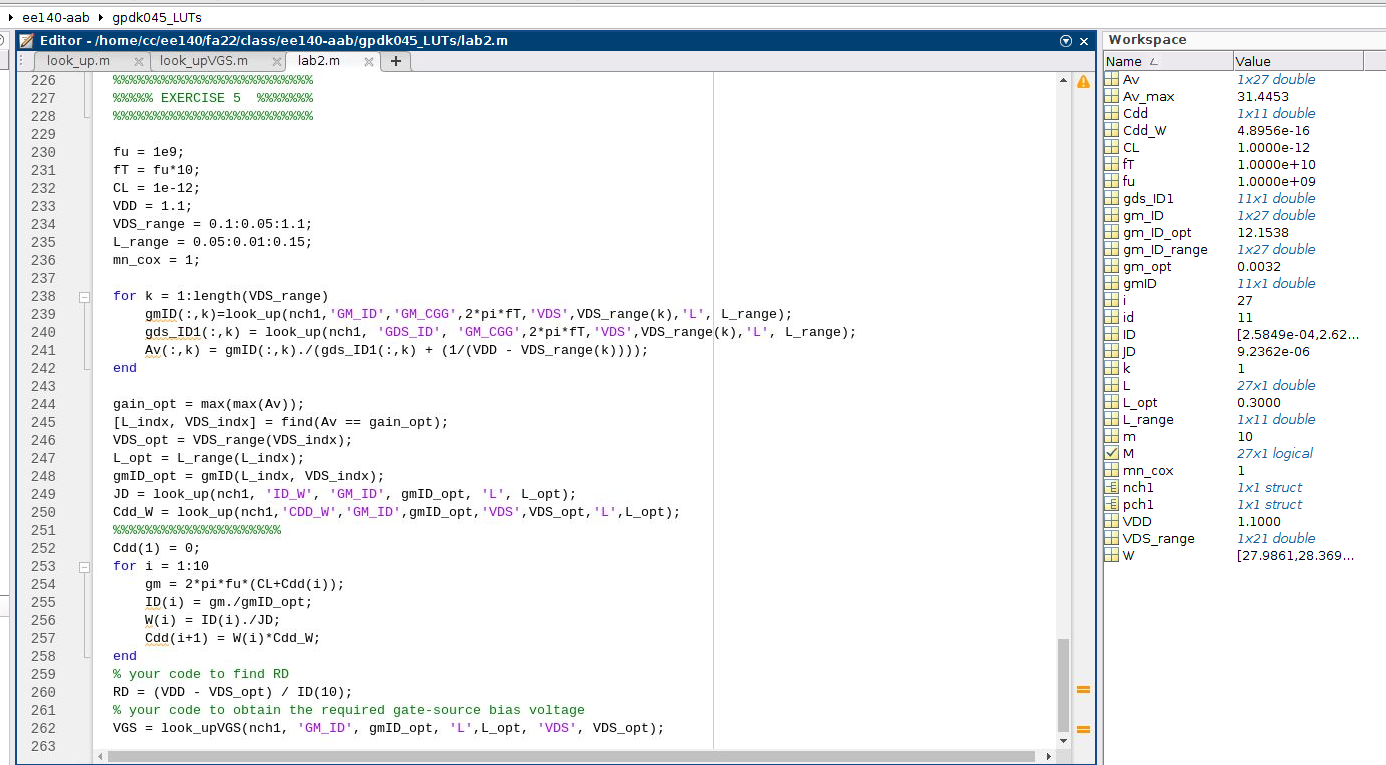
\includegraphics[scale=0.375, center]{mat_res9.PNG}\\[0.25cm]
\newpage
The gain was around 6 with the value for $V_{GS}$ from MATLAB.  I swept the gain as a function of $V_{GS}$ to find the optimum operating point.  Below is the plot used:\\[0.25cm]
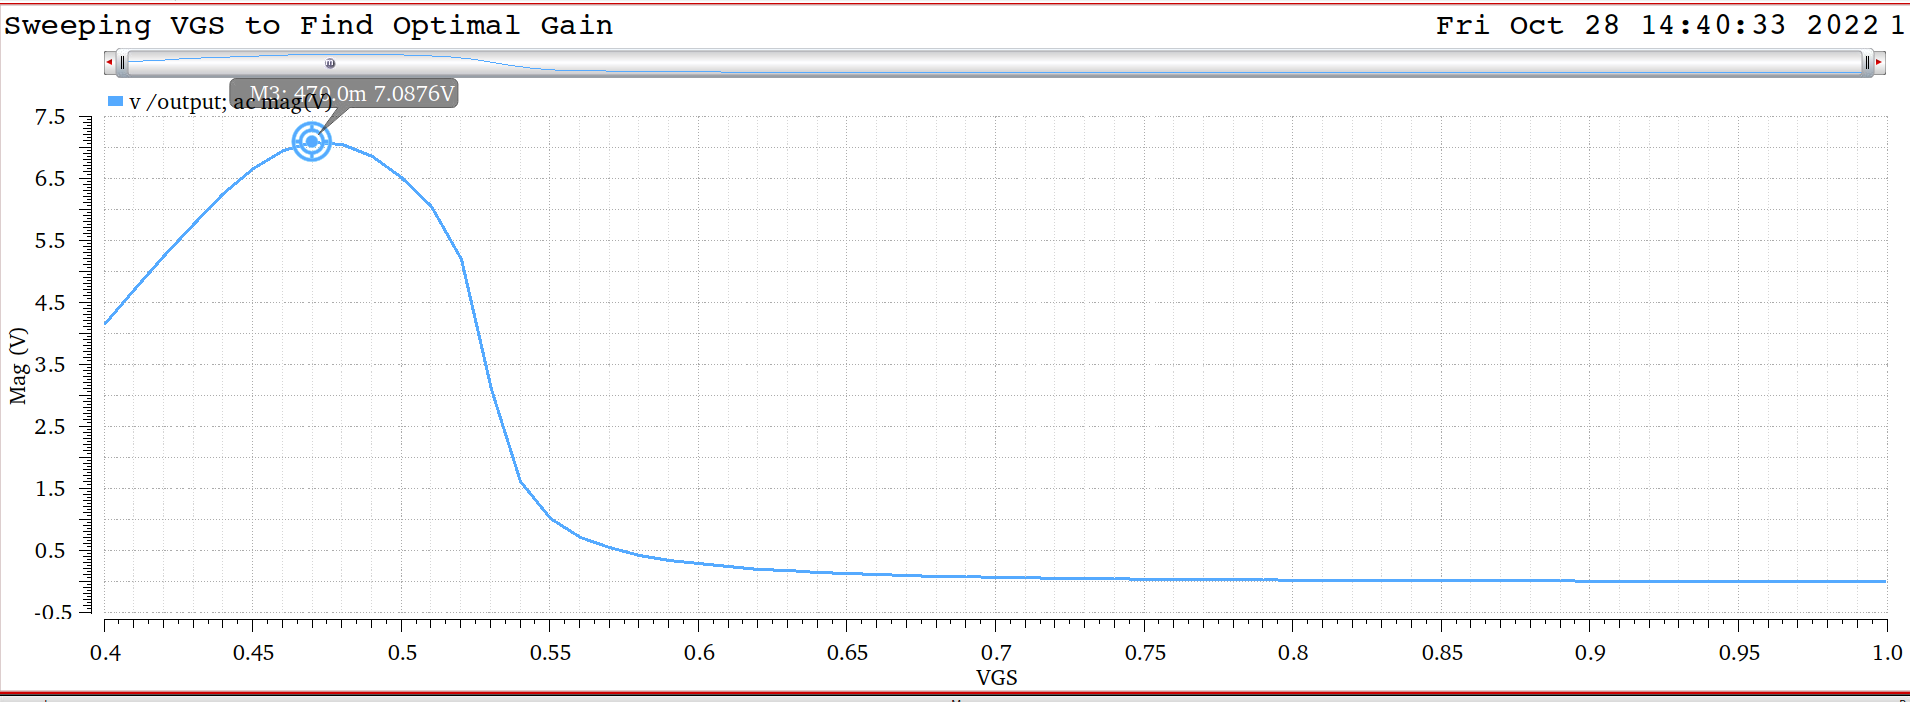
\includegraphics[scale=0.275, center]{opt_vgs.PNG}\\[0.25cm]
This fixed the gain, and all other parameters now match the results from MATLAB.  Below is the circuit schematic with node voltages and currents:\\[0.25cm]
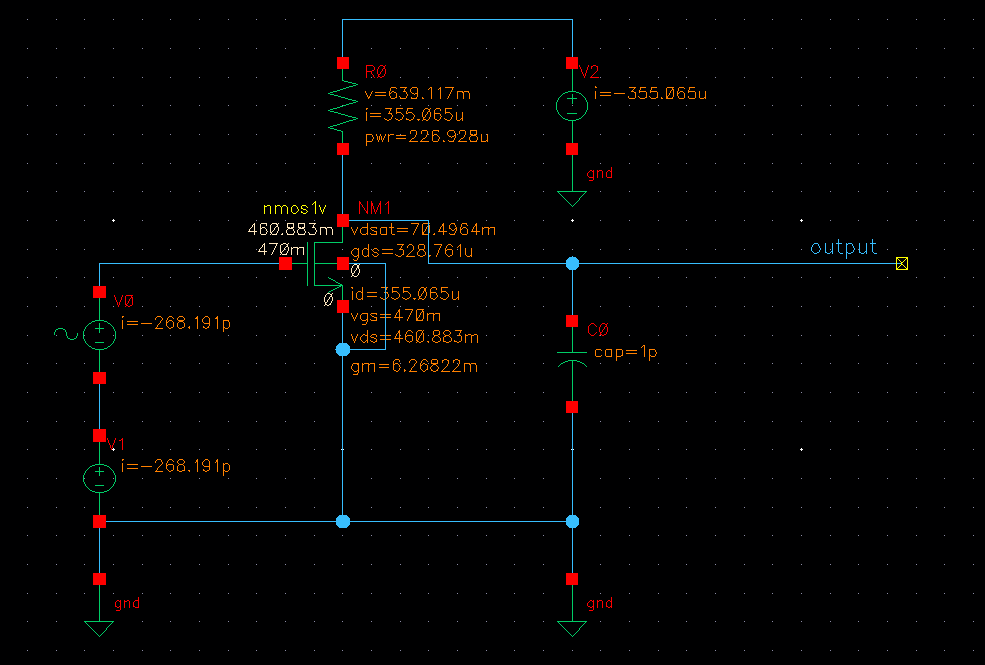
\includegraphics[scale=0.35, center]{schem7.PNG}\\[0.25cm]
Below is the new simulation results:\\[0.25cm]
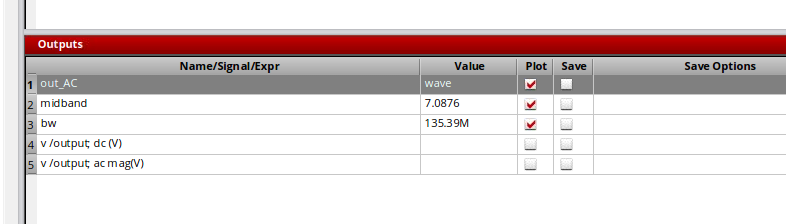
\includegraphics[scale=0.375, center]{sim_res8.PNG}\\[0.25cm]
\newpage
Below is the new Bode plot with the unity gain frequency marked:\\[0.25cm]
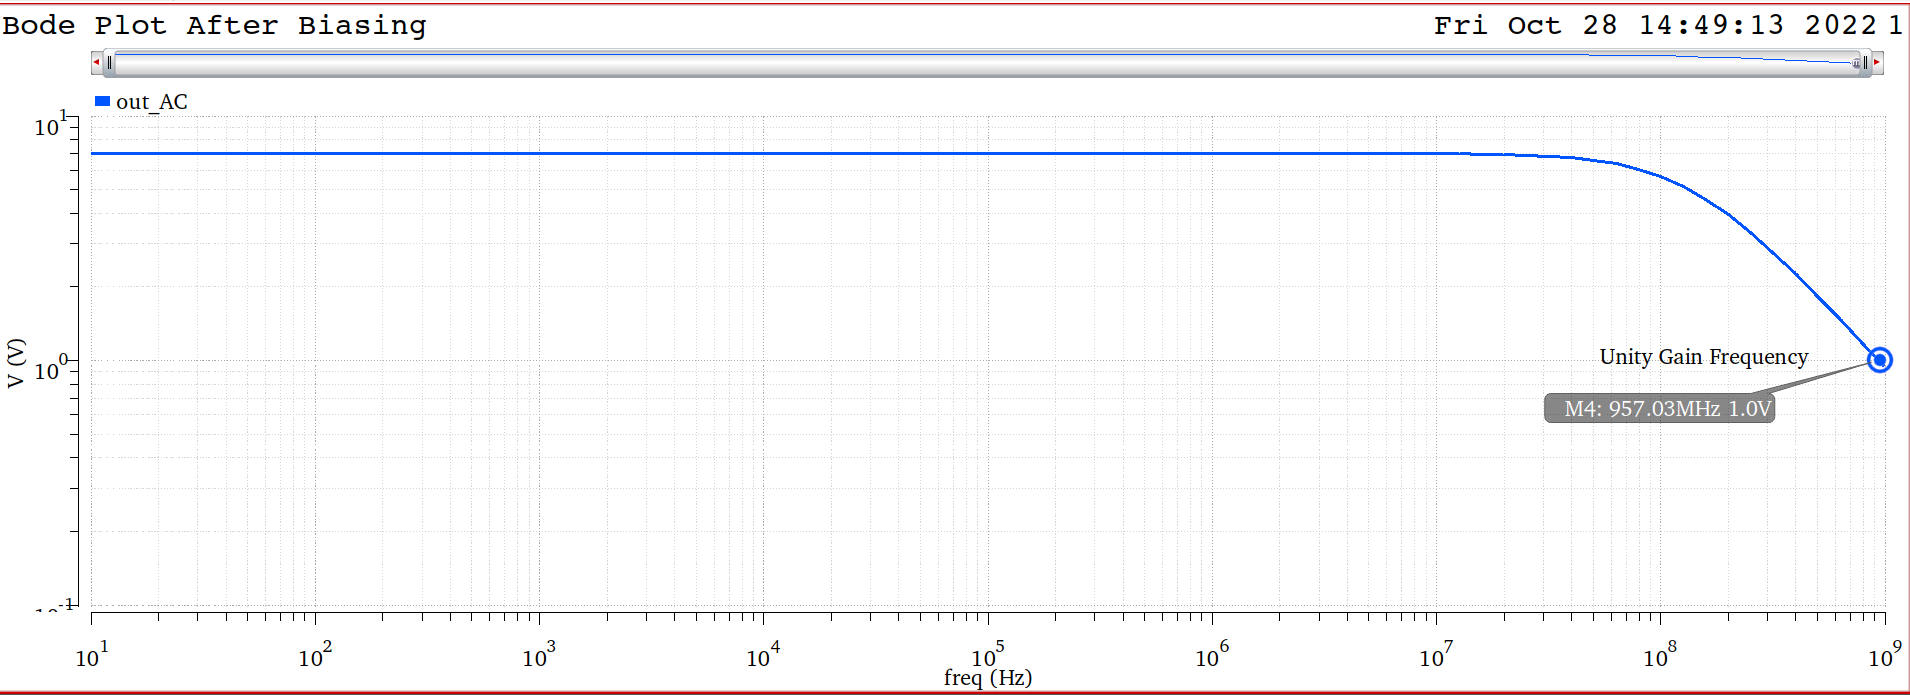
\includegraphics[scale=0.275, center]{bode8.PNG}\\[0.25cm]
Now we will set the unity gain frequency to 100 MHz in order to match the circuit from Lab 0, and then do the same process as before (thus, pictures of finding the operating point will be omitted).  Below is the new MATLAB results:\\[0.25cm]
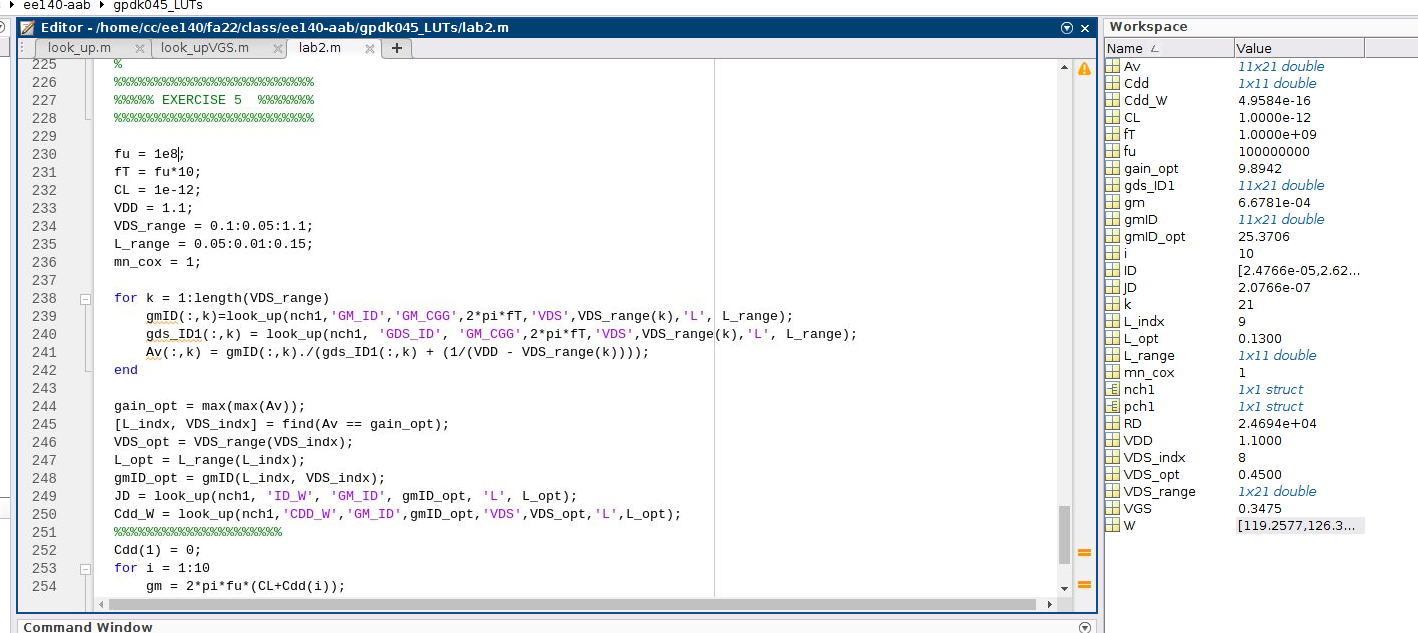
\includegraphics[scale=0.375, center]{mat_res10.PNG}\\[0.25cm]
\newpage
Below is the circuit schematic with node voltages and currents:\\[0.25cm]
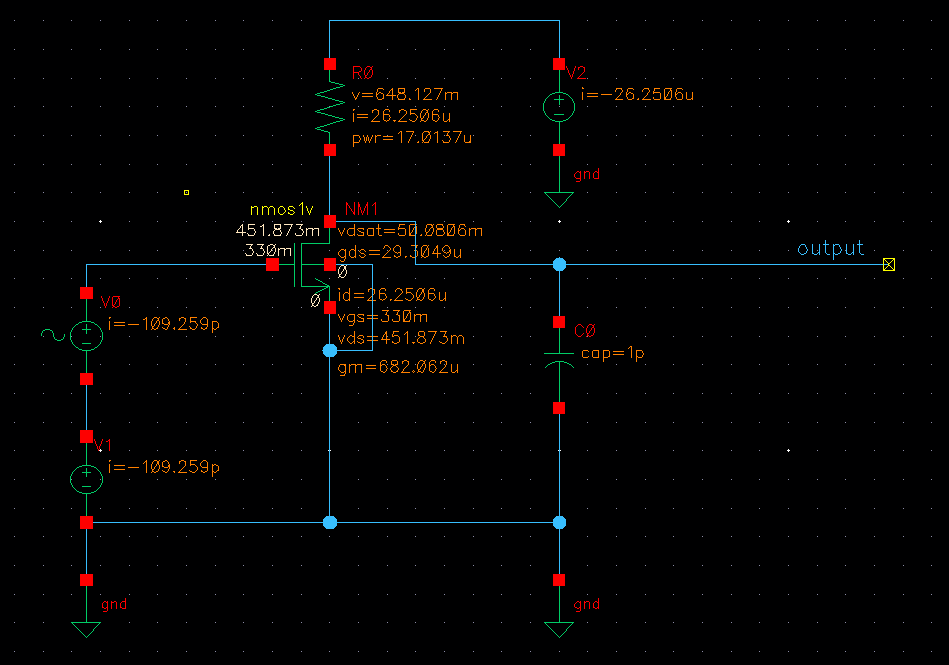
\includegraphics[scale=0.375, center]{schem8.PNG}\\[0.25cm]
\newpage
Below is the new simulation results:\\[0.25cm]
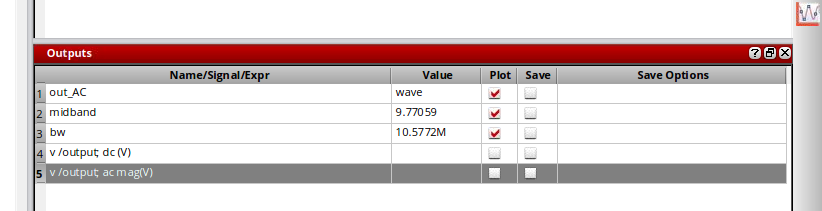
\includegraphics[scale=0.375, center]{sim_res9.PNG}\\[0.25cm]
Below is the Bode plot with the unity gain frequency marked:\\[0.25cm]
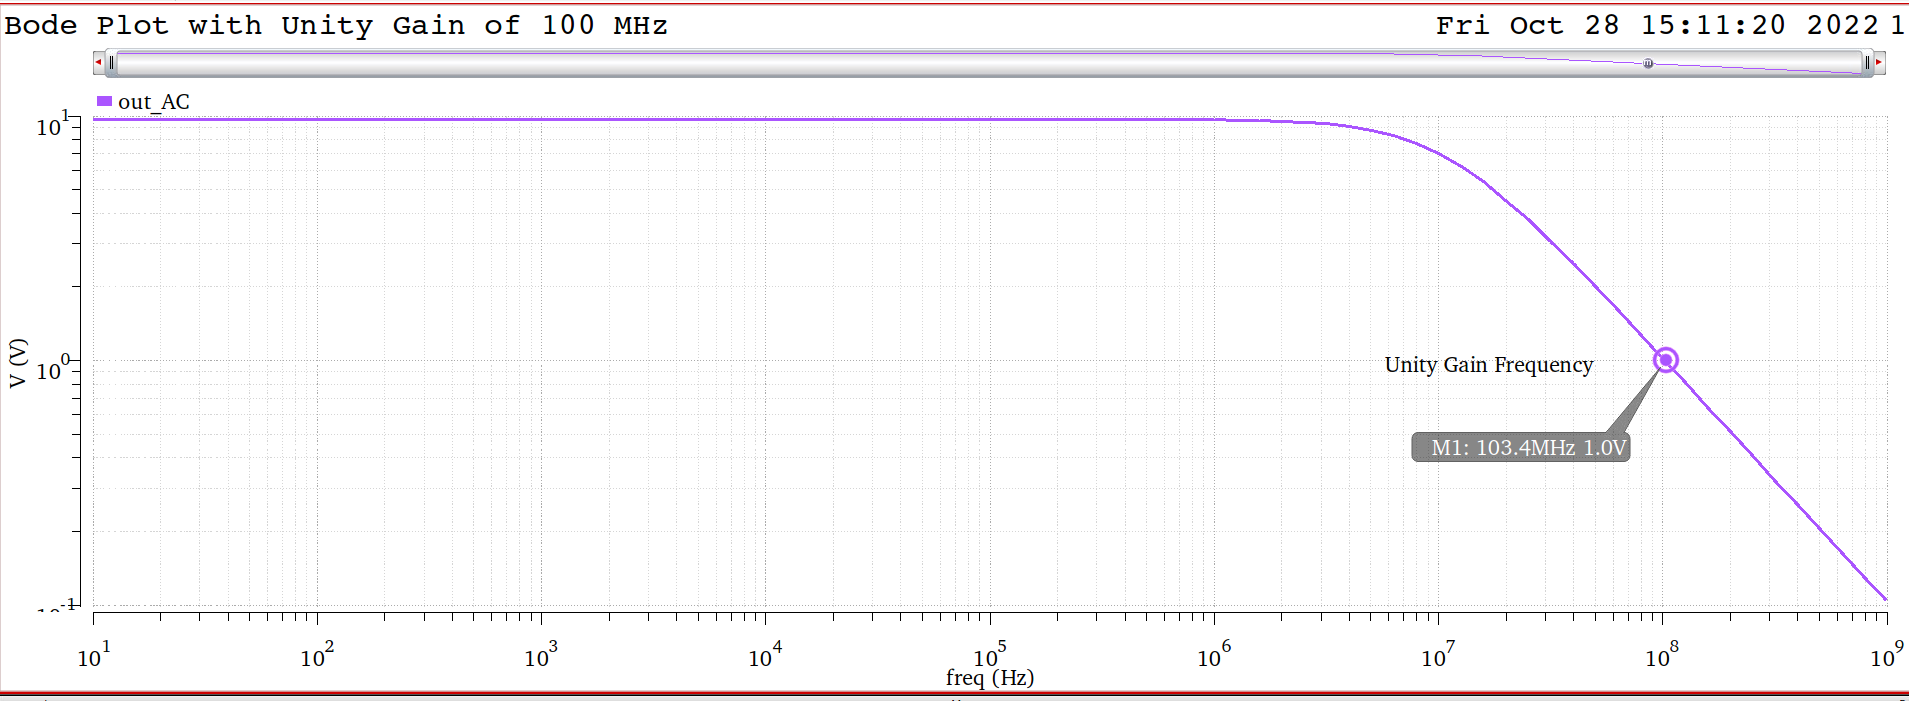
\includegraphics[scale=0.275, center]{bode9.PNG}\\[0.25cm]
Below is a table comparing the performance results of both schematics.
    \begin{table}[H]
    \centering
    \setlength{\tabcolsep}{8pt}
    \renewcommand{\arraystretch}{1.5}
        \begin{tabular}{|c|c|c|c|}
            \hline
            \textbf{Parameter} & \textit{Lab 0 Amp} & \textit{Ex. 5 Amp w/} $f_u = 1\,GHz$ & \textit{Ex. 5 Amp w/} $f_u = 100\,MHz$\\
            \hline
            $A_v\;(V/V)$ & $3.938$ & $7.0876$ & $9.77059$\\
            \hline
            $BW\;(MHz)$ & $24.5322$ & $135.39$ & $10.577$\\
            \hline
            $f_u\;(MHz)$ & $94.4547$ & $957.03$ & $103.4$\\
            \hline
            $W (\mu m)$ & $2$ & $89.7548$ & $126.753$\\
            \hline
            $L (\mu m)$ & $0.1$ & $0.11$ & $0.13$\\
            \hline
            $V_{DS} (V)$ & $0.66$ & $0.461$ & $0.45$\\
            \hline
            $R_D (\Omega)$ & $7.8\,k$ & $1.81k$ & $24.7\,k$\\
            \hline
            $Power (\mu Watts)$ & $61.43$ & $390.5715$ & $28.88$\\
            \hline
        \end{tabular}
    \end{table}
\newpage
%%%%%%%%%%%%%%%%%%%%%%%%%%%%%%%%%%%%%%%%%%%%%%%%%%%%%%%%%%%%%%%%%%%%%%%%%%%%%%%%%%%%%%%%%%%%%%%%%%%%%%%%%%%
%                                             APPENDIX                                                    %
%%%%%%%%%%%%%%%%%%%%%%%%%%%%%%%%%%%%%%%%%%%%%%%%%%%%%%%%%%%%%%%%%%%%%%%%%%%%%%%%%%%%%%%%%%%%%%%%%%%%%%%%%%%
\appendix
%%%%%%%%%%%%%%%%%%%%%%%%%%%%%%%%%%%%%%%%%%%%%%%%%%%%%%%%%%%%%%%%%%%%%%%%%%%%%%%%%%%%%%%%%%%%%%%%%%%%%%%%%%%
%                                APPENDIX A: GLOSSARY OF EQUATIONS                                        %
%%%%%%%%%%%%%%%%%%%%%%%%%%%%%%%%%%%%%%%%%%%%%%%%%%%%%%%%%%%%%%%%%%%%%%%%%%%%%%%%%%%%%%%%%%%%%%%%%%%%%%%%%%%
\newpage
\section{Appendix: Glossary of Equations}
    \begin{flalign}
        &&\Aboxed{\phi_{bi} &= \frac{kT}{q} \cdot ln\;\bigg( \frac{N_D \cdot N_A}{{n_i}^2} \bigg)}
        &&\textit{Built-in potential, $PN$-junction}
        \label{eq:phi_bi}
    \end{flalign}

    \begin{flalign}
        &&\Aboxed{W_{dep} &= \sqrt{\frac{2\epsilon_s \left(\phi_{bi} - V_{applied}\right)}{q}
                        \cdot \Bigg( \frac{1}{N_A} + \frac{1}{N_D} \Bigg)}}
        &&\textit{Depletion region width, total}
        \label{eq:total_dep}
    \end{flalign}        

    \begin{flalign}
        &&\Aboxed{C_{dep} &= A \left(\frac{\epsilon_s}{W_{dep}}\right)}
        &&\textit{Junction capacitance}
        \label{eq:junc_cap}
    \end{flalign}

    \begin{flalign}
        &&\Aboxed{I_{DS,sat} &= \left(\frac{W}{2L}\right) \mu_n\,C_{ox}
                         {\big(V_{GS} - V_{T_n}\big)}^2 (1 + \lambda V_{DS})}
        &&\textit{$NMOS$ saturation current}
        \label{eq:mosfet_ids_nmos_sat}\\[0.25cm]
        &&\Aboxed{I_{DS,tri} &= \left(\frac{W}{L}\right) \mu_n\,C_{ox}
                            \left(V_{GS} - V_{T_n} - \frac{V_{DS}}{2}\right) V_{DS}}
        &&\textit{$NMOS$ triode current}
        \label{eq:mosfet_ids_nmos_tri}\\[0.25cm]
        &&\Aboxed{I_{SD,sat} &= \left(\frac{W}{2L}\right) \mu_p\,C_{ox}
                         {\big(V_{SG} - \left|V_{T_p}\right|\big)}^2 (1 + \lambda V_{SD})}
        &&\textit{$PMOS$ saturation current}
        \label{eq:mosfet_ids_pmos_sat}\\[0.25cm]
        &&\Aboxed{I_{SD,tri} &= \left(\frac{W}{L}\right) \mu_p\,C_{ox}
                            \left(V_{SG} - \left|V_{T_p}\right| - \frac{V_{SD}}{2}\right) V_{SD}}
        &&\textit{$PMOS$ triode current}
        \label{eq:mosfet_ids_pmos_tri}
    \end{flalign}

    \begin{flalign}
        &&\Aboxed{r_o &= \frac{1}{\frac{W\,\mu\,C_{ox}}{2L}{(V_{GS} - V_T)}^2\,\lambda}
        \approx \frac{1}{\lambda\,I_{DS}}}
        &&\textit{Output resistance for MOSFET}
        \label{eq:mos_outresistance}
    \end{flalign}

    \begin{flalign}
        &&\Aboxed{g_m &= \left(\frac{W}{L}\right)\mu\,C_{ox}(V_{{DS}_{sat}})
        = \sqrt{\left(\frac{2W}{L}\right)\mu\,C_{ox} I_{DS}}
        = \frac{2 \cdot I_{DS}}{V_{GS} - V_T}}
        &&\textit{Transconductance for MOSFET}
        \label{eq:mos_transconductance}
    \end{flalign}

    \begin{flalign}
        &&\Aboxed{V_{GS} = V_T + \sqrt{\frac{2\,I_{DS}}{\frac{W}{L} \mu C_{ox}}} = V_T + V_{OD}}
        &&\textit{Gate-source condition, diode-connected MOSFET}
        \label{eq:mos_gate_cond}
    \end{flalign}
%%%%%%%%%%%%%%%%%%%%%%%%%%%%%%%%%%%%%%%%%%%%%%%%%%%%%%%%%%%%%%%%%%%%%%%%%%%%%%%%%%%%%%%%%%%%%%%%%%%%%%%%%%%
%                                APPENDIX B: GLOSSARY OF TABLES                                           %
%%%%%%%%%%%%%%%%%%%%%%%%%%%%%%%%%%%%%%%%%%%%%%%%%%%%%%%%%%%%%%%%%%%%%%%%%%%%%%%%%%%%%%%%%%%%%%%%%%%%%%%%%%%
\newpage
\section{Appendix: Glossary of Tables}
    \begin{table}[H]
    \centering
    \setlength{\tabcolsep}{20pt}
    \renewcommand{\arraystretch}{1.5}
    \begin{tabular}{|l|c|c|c|}
        \hline
        \textbf{Transistor Type}  &  \textbf{Cut-off} & \textbf{Triode} & \textbf{Saturation}\\
        \hline
        \textit{NMOS} & $V_{GS} \leq V_{T_n}$
                        & $V_{DS} \leq V_{GS} - V_{T_n}$
                        & $V_{DS} > V_{GS} - V_{T_n}$\\
        \hline
        \textit{PMOS} & $V_{SG} \leq \left|V_{T_p}\right|$
                        & $V_{SD} \leq V_{SG} - \left|V_{T_p}\right|$
                        & $V_{SD} > V_{SG} - \left|V_{T_p}\right|$\\
        \hline
    \end{tabular}
    \caption{Conditions for MOSFET regions of operation.
    \label{tab:mosfet_op}} 
    \end{table}

    \begin{table}[H]
    \centering
    \setlength{\tabcolsep}{20pt}
    \renewcommand{\arraystretch}{1.5}
    \begin{tabular}{|l|c|c|}
        \hline
        \textbf{Description}  &  \textbf{Symbol} & \textbf{Value}\\
        \hline
        Elementary charge & $q$ & $\num{1.60218e-19}\,C$\\
        \hline
        Electron volt & $eV$ & $\num{1.60218e-19}\,J$\\
        \hline
        Boltzmann's constant & $k$ & $\num{1.38066e-23}\,J/K$\\
        \hline
        Free electron mass & $m_0$ & $\num{9.1095e-31}\,kg$\\
        \hline
        Permittivity in vacuum & $\epsilon_0$ & $\num{8.85418e-12}\,F/m$\\
        \hline
        Planck's constant & $h$ & $\num{6.62617e-34}\,J \cdot s$\\
        \hline
        Reduced Planck's constant ($h/2\pi$) & $\hbar$ & $\num{1.05458e-34}\,J \cdot s$\\
        \hline
        Speed of light in vacuum & $c$ & $\num{2.99792e8}\,m/s$\\
        \hline
        Thermal voltage at $T=300^{\circ}K$ & $kT/q$ & $0.0259\,V$\\
        \hline
        Wavelength of 1-$eV$ photon & $\lambda$ & $1.23977\,\mu m$\\
        \hline
    \end{tabular}
    \caption{Physical constants.
    \label{tab:phys_const}} 
    \end{table}
\newpage
    \begin{table}[H]
    \centering
    \setlength{\tabcolsep}{20pt}
    \renewcommand{\arraystretch}{1.5}
    \begin{tabular}{|l|c|c|}
        \hline
        \textbf{Quantity}  &  \textbf{Symbol} & \textbf{Value/Dimension}\\
        \hline
        Meter & $m$ & $1\,m = 10^2\,cm$\\
        \hline
        Millimeter & $mm$ & $1\,mm = 10^{-1}\,cm = 10^{-3}\,m$\\
        \hline
        Micrometer, micron & $\mu m$ & $1\,\mu m = 10^4\,\text{\AA} = 10^3\,mm = 10^{-4}\,cm$\\
        \hline
        Nanometer & $nm$ & $1\,nm = 10\,\text{\AA} = 10^{-3}\,\mu m = 10^{-7}\,cm$\\
        \hline
        Angstrom & $\text{\AA}$ & $1\,\text{\AA} = 10^{-4}\,\mu m = 10^{-8}\,cm = 10^{-10}\,m$\\
        \hline
        Electron volt & $eV$ & $1\,eV = \num{1.60218e-19}\,J$\\
        \hline
        Electric charge (Coulomb) & $C$ & $A \cdot s$\\
        \hline
        Current (Ampere) & $A$ & $C/s$\\
        \hline
        Frequency (Hertz) & $Hz$ & $1/s$\\
        \hline
        Energy (Joule) & $J$ & $N \cdot m$\\
        \hline
        Power (Watt) & $W$ & $J/s$\\
        \hline
        Potential (Volt) & $V$ & $J/C$\\
        \hline
        Conductance (Siemens) & $S$ & $A/V$\\
        \hline
        Resistance (Ohm) & $\Omega$ & $V/A$\\
        \hline
        Capacitance (Farad) & $F$ & $C/V$\\
        \hline
    \end{tabular}
    \caption{Unit conversions.
    \label{tab:unit_conv}} 
    \end{table}
\newpage
%%%%%%%%%%%%%%%%%%%%%%%%%%%%%%%%%%%%%%%%%%%%%%%%%%%%%%%%%%%%%%%%%%%%%%%%%%%%%%%%%%%%%%%%%%%%%%%%%%%%%%%%%%%
%                                           BIBLIOGRAPHY                                                  %
%%%%%%%%%%%%%%%%%%%%%%%%%%%%%%%%%%%%%%%%%%%%%%%%%%%%%%%%%%%%%%%%%%%%%%%%%%%%%%%%%%%%%%%%%%%%%%%%%%%%%%%%%%%
\newpage
\addcontentsline{toc}{section}{References}
\emergencystretch=2em
\nocite{*}
\printbibliography
%%%%%%%%%%%%%%%%%%%%%%%%%%%%%%%%%%%%%%%%%%%%%%%%%%%%%%%%%%%%%%%%%%%%%%%%%%%%%%%%%%%%%%%%%%%%%%%%%%%%%%%%%%%
%                                           END OF DOCUMENT                                               %
%%%%%%%%%%%%%%%%%%%%%%%%%%%%%%%%%%%%%%%%%%%%%%%%%%%%%%%%%%%%%%%%%%%%%%%%%%%%%%%%%%%%%%%%%%%%%%%%%%%%%%%%%%%
\end{document}
